Στο σχήμα \ref{fig:02_05_04:01} απεικονίζεται η διαδικασία ευθυγράμμισης δύο
πανοραμικών δισδιάστατων σαρώσεων που συνελήφθησαν σε ένα περιβάλλον του συνόλου
δεδομένων \texttt{laserazos}\footref{foot:laserazos} μέσω των μεθόδων FastGICP
και FSM.  Εδώ παρατηρούμε πως ο πρώτος---όπως και όλες οι εκδόσεις του
ICP---εκτιμούν σταδιακά τον προσανατολισμό ανάμεσα στις δύο στάσεις από τις
οποίες συνελήφθησαν οι δύο σαρώσεις, σε αντίθεση με τον FSM, ο οποίος το κάνει
σε ένα βήμα---και από εκεί και πέρα παρέχει όλο και πιο ακριβείς εκτιμήσεις μέσω
της υπερδειγματοληψίας του χάρτη $\widetilde{\bm{M}}$. Ο FastGICP χρησιμοποιεί
αντιστοιχίσεις για τα δύο σκέλη της ευθυγράμμισης, και ως εσωτερική μετρική το
μέτρο της εξ. (\ref{eq:sm_def}), ενώ ο FSM δεν χρησιμοποιεί αντιστοιχίσεις
όλως διόλου, και η εσωτερική μετρική του είναι η μετρική CAER (εξ.
(\ref{eq:caer_normal}), όπου $\mathcal{S}_R \leftarrow \mathcal{S}_1$,
$\mathcal{S}_V \leftarrow \mathcal{S}_0$, $(x,y,\theta)\leftarrow\bm{p}_1$, και
$(\hat{x}, \hat{y}, \hat{\theta}) \leftarrow \bm{p}_0$). Από τα αποτελέσματα
παρατηρούμε πως το σφάλμα εκτίμησης θέσης του FastGICP δεν ακολουθεί την
(μειούμενη) τροχιά της εσωτερικής του μετρικής---σε αντίθεση με αυτό του
FSM---και πως αυξάνει προτού στη συνέχεια μειωθεί, με αποτέλεσμα την
παγίδευση της εκτίμησης θέσης σε τοπικό ελάχιστο. Δεδομένου ότι οι συχνότητα
ανανέωσης μετρήσεων από τους εμπορικά διαθέσιμους πανοραμικούς αισθητήρες lidar
κυμαίνεται από $10$ έως $20$ Hz, με βάση την απόσταση των στάσεων από τις οποίες
συνελήφθησαν οι δύο μετρήσεις, συμπεραίνουμε πως ο FSM είναι ικανός εκτίμησης
της τροχιάς ενός ρομπότ το οποίο κινείται με ακτινική ταχύτητα $7.28$ m/s
($\simeq 25$ km/h).

\begin{figure}[]\centering
  \definecolor{pp}{RGB}{127,201,127}
\definecolor{cc}{RGB}{0,0,0}
\definecolor{oo}{RGB}{251,128,114}

% GNUPLOT: LaTeX picture with Postscript
\begingroup
  \makeatletter
  \providecommand\color[2][]{%
    \GenericError{(gnuplot) \space\space\space\@spaces}{%
      Package color not loaded in conjunction with
      terminal option `colourtext'%
    }{See the gnuplot documentation for explanation.%
    }{Either use 'blacktext' in gnuplot or load the package
      color.sty in LaTeX.}%
    \renewcommand\color[2][]{}%
  }%
  \providecommand\includegraphics[2][]{%
    \GenericError{(gnuplot) \space\space\space\@spaces}{%
      Package graphicx or graphics not loaded%
    }{See the gnuplot documentation for explanation.%
    }{The gnuplot epslatex terminal needs graphicx.sty or graphics.sty.}%
    \renewcommand\includegraphics[2][]{}%
  }%
  \providecommand\rotatebox[2]{#2}%
  \@ifundefined{ifGPcolor}{%
    \newif\ifGPcolor
    \GPcolorfalse
  }{}%
  \@ifundefined{ifGPblacktext}{%
    \newif\ifGPblacktext
    \GPblacktexttrue
  }{}%
  % define a \g@addto@macro without @ in the name:
  \let\gplgaddtomacro\g@addto@macro
  % define empty templates for all commands taking text:
  \gdef\gplfronttext{}%
  \gdef\gplfronttext{}%
  \makeatother
  \ifGPblacktext
    % no textcolor at all
    \def\colorrgb#1{}%
    \def\colorgray#1{}%
  \else
    % gray or color?
    \ifGPcolor
      \def\colorrgb#1{\color[rgb]{#1}}%
      \def\colorgray#1{\color[gray]{#1}}%
      \expandafter\def\csname LTw\endcsname{\color{white}}%
      \expandafter\def\csname LTb\endcsname{\color{black}}%
      \expandafter\def\csname LTa\endcsname{\color{black}}%
      \expandafter\def\csname LT0\endcsname{\color[rgb]{1,0,0}}%
      \expandafter\def\csname LT1\endcsname{\color[rgb]{0,1,0}}%
      \expandafter\def\csname LT2\endcsname{\color[rgb]{0,0,1}}%
      \expandafter\def\csname LT3\endcsname{\color[rgb]{1,0,1}}%
      \expandafter\def\csname LT4\endcsname{\color[rgb]{0,1,1}}%
      \expandafter\def\csname LT5\endcsname{\color[rgb]{1,1,0}}%
      \expandafter\def\csname LT6\endcsname{\color[rgb]{0,0,0}}%
      \expandafter\def\csname LT7\endcsname{\color[rgb]{1,0.3,0}}%
      \expandafter\def\csname LT8\endcsname{\color[rgb]{0.5,0.5,0.5}}%
    \else
      % gray
      \def\colorrgb#1{\color{black}}%
      \def\colorgray#1{\color[gray]{#1}}%
      \expandafter\def\csname LTw\endcsname{\color{white}}%
      \expandafter\def\csname LTb\endcsname{\color{black}}%
      \expandafter\def\csname LTa\endcsname{\color{black}}%
      \expandafter\def\csname LT0\endcsname{\color{black}}%
      \expandafter\def\csname LT1\endcsname{\color{black}}%
      \expandafter\def\csname LT2\endcsname{\color{black}}%
      \expandafter\def\csname LT3\endcsname{\color{black}}%
      \expandafter\def\csname LT4\endcsname{\color{black}}%
      \expandafter\def\csname LT5\endcsname{\color{black}}%
      \expandafter\def\csname LT6\endcsname{\color{black}}%
      \expandafter\def\csname LT7\endcsname{\color{black}}%
      \expandafter\def\csname LT8\endcsname{\color{black}}%
    \fi
  \fi
    \setlength{\unitlength}{0.0500bp}%
    \ifx\gptboxheight\undefined%
      \newlength{\gptboxheight}%
      \newlength{\gptboxwidth}%
      \newsavebox{\gptboxtext}%
    \fi%
    \setlength{\fboxrule}{0.5pt}%
    \setlength{\fboxsep}{1pt}%
\begin{picture}(8000.00,8000.00)%
    \gplgaddtomacro\gplfronttext{%
    }%
    \gplgaddtomacro\gplfronttext{%
      \colorrgb{0.00,0.00,0.00}%
      \put(3999,7959){\makebox(0,0){\strut{}\small Αρχική συνθήκη}}%
      \put(600, 3770){\makebox(0,0){\strut{}{\color{pp}{\rule[0.6mm]{0.5cm}{0.5mm}}} \small Σφάλμα θέσης [m]}}
      \put(3420,3770){\makebox(0,0){\strut{}{\color{oo}{\rule[0.6mm]{0.5cm}{0.5mm}}} \small Σφάλμα προσανατολισμού [rad]}}
      \put(7020,3770){\makebox(0,0){\strut{}{\color{cc}{\rule[0.6mm]{0.5cm}{0.5mm}}} \small Οικεία εσωτερική μετρική σφάλματος [m]}}
    }%
    \gplgaddtomacro\gplfronttext{%
    }%
    \gplgaddtomacro\gplfronttext{%
      \colorrgb{0.00,0.00,0.00}%
      \put(1839,5959){\makebox(0,0){\strut{}\small Εξέλιξη ευθυγράμμισης FastGICP}}%
    }%
    \gplgaddtomacro\gplfronttext{%
    }%
    \gplgaddtomacro\gplfronttext{%
      \colorrgb{0.00,0.00,0.00}%
      \put(6159,5959){\makebox(0,0){\strut{}\small Εξέλιξη ευθυγράμμισης \texttt{fsm}}}%
    }%
    \gplgaddtomacro\gplfronttext{%
      \colorrgb{0.00,0.45,0.74}%
      \put(508,2400){\makebox(0,0)[r]{\strut{}\scriptsize $0.0$}}%
      \colorrgb{0.00,0.45,0.74}%
      \put(508,2543){\makebox(0,0)[r]{\strut{}\scriptsize $0.2$}}%
      \colorrgb{0.00,0.45,0.74}%
      \put(508,2685){\makebox(0,0)[r]{\strut{}\scriptsize $0.4$}}%
      \colorrgb{0.00,0.45,0.74}%
      \put(508,2828){\makebox(0,0)[r]{\strut{}\scriptsize $0.6$}}%
      \colorrgb{0.00,0.45,0.74}%
      \put(508,2971){\makebox(0,0)[r]{\strut{}\scriptsize $0.8$}}%
      \colorrgb{0.00,0.45,0.74}%
      \put(508,3114){\makebox(0,0)[r]{\strut{}\scriptsize $1.0$}}%
      \colorrgb{0.00,0.45,0.74}%
      \put(508,3256){\makebox(0,0)[r]{\strut{}\scriptsize $1.2$}}%
      \colorrgb{0.00,0.45,0.74}%
      \put(508,3399){\makebox(0,0)[r]{\strut{}\scriptsize $1.4$}}%
    }%
    \gplgaddtomacro\gplfronttext{%
    }%
    \gplgaddtomacro\gplfronttext{%
      \colorrgb{0.15,0.15,0.15}%
      \put(640,2180){\makebox(0,0){\strut{}\scriptsize $0$}}%
      \colorrgb{0.15,0.15,0.15}%
      \put(1089,2180){\makebox(0,0){\strut{}\scriptsize $10$}}%
      \colorrgb{0.15,0.15,0.15}%
      \put(1538,2180){\makebox(0,0){\strut{}\scriptsize $20$}}%
      \colorrgb{0.85,0.33,0.10}%
      \put(1715,2400){\makebox(0,0)[l]{\strut{}}}%
      \colorrgb{0.85,0.33,0.10}%
      \put(1715,2600){\makebox(0,0)[l]{\strut{}}}%
      \colorrgb{0.85,0.33,0.10}%
      \put(1715,2800){\makebox(0,0)[l]{\strut{}}}%
      \colorrgb{0.85,0.33,0.10}%
      \put(1715,2999){\makebox(0,0)[l]{\strut{}}}%
      \colorrgb{0.85,0.33,0.10}%
      \put(1715,3199){\makebox(0,0)[l]{\strut{}}}%
      \colorrgb{0.85,0.33,0.10}%
      \put(1715,3399){\makebox(0,0)[l]{\strut{}}}%
    }%
    \gplgaddtomacro\gplfronttext{%
    }%
    \gplgaddtomacro\gplfronttext{%
      \colorrgb{1.00,0.00,1.00}%
      \put(2108,2400){\makebox(0,0)[r]{\strut{}\scriptsize $0$}}%
      \colorrgb{1.00,0.00,1.00}%
      \put(2108,2574){\makebox(0,0)[r]{\strut{}\scriptsize $0.18$}}%
      \colorrgb{1.00,0.00,1.00}%
      \put(2108,2749){\makebox(0,0)[r]{\strut{}\scriptsize $0.35$}}%
      \colorrgb{1.00,0.00,1.00}%
      \put(2108,2923){\makebox(0,0)[r]{\strut{}\scriptsize $0.52$}}%
      \colorrgb{1.00,0.00,1.00}%
      \put(2108,3097){\makebox(0,0)[r]{\strut{}\scriptsize $0.70$}}%
      \colorrgb{1.00,0.00,1.00}%
      \put(2108,3272){\makebox(0,0)[r]{\strut{}\scriptsize $0.87$}}%
    }%
    \gplgaddtomacro\gplfronttext{%
    }%
    \gplgaddtomacro\gplfronttext{%
      \colorrgb{0.15,0.15,0.15}%
      \put(2240,2180){\makebox(0,0){\strut{}\scriptsize $0$}}%
      \colorrgb{0.15,0.15,0.15}%
      \put(2689,2180){\makebox(0,0){\strut{}\scriptsize $10$}}%
      \colorrgb{0.15,0.15,0.15}%
      \put(3138,2180){\makebox(0,0){\strut{}\scriptsize $20$}}%
      \colorrgb{0.85,0.33,0.10}%
      \put(3315,2400){\makebox(0,0)[l]{\strut{}\scriptsize $0$}}%
      \colorrgb{0.85,0.33,0.10}%
      \put(3315,2600){\makebox(0,0)[l]{\strut{}\scriptsize $100$}}%
      \colorrgb{0.85,0.33,0.10}%
      \put(3315,2800){\makebox(0,0)[l]{\strut{}\scriptsize $200$}}%
      \colorrgb{0.85,0.33,0.10}%
      \put(3315,2999){\makebox(0,0)[l]{\strut{}\scriptsize $300$}}%
      \colorrgb{0.85,0.33,0.10}%
      \put(3315,3199){\makebox(0,0)[l]{\strut{}\scriptsize $400$}}%
      \colorrgb{0.85,0.33,0.10}%
      \put(3315,3399){\makebox(0,0)[l]{\strut{}\scriptsize $500$}}%
    }%
    \gplgaddtomacro\gplfronttext{%
    }%
    \gplgaddtomacro\gplfronttext{%
      \colorrgb{0.00,0.45,0.74}%
      \put(4668,2400){\makebox(0,0)[r]{\strut{}\scriptsize $0.0$}}%
      \colorrgb{0.00,0.45,0.74}%
      \put(4668,2650){\makebox(0,0)[r]{\strut{}\scriptsize $0.1$}}%
      \colorrgb{0.00,0.45,0.74}%
      \put(4668,2900){\makebox(0,0)[r]{\strut{}\scriptsize $0.2$}}%
      \colorrgb{0.00,0.45,0.74}%
      \put(4668,3149){\makebox(0,0)[r]{\strut{}\scriptsize $0.3$}}%
      \colorrgb{0.00,0.45,0.74}%
      \put(4668,3399){\makebox(0,0)[r]{\strut{}\scriptsize $0.4$}}%
    }%
    \gplgaddtomacro\gplfronttext{%
    }%
    \gplgaddtomacro\gplfronttext{%
      \colorrgb{0.15,0.15,0.15}%
      \put(5010,2180){\makebox(0,0){\strut{}\scriptsize $2$}}%
      \colorrgb{0.15,0.15,0.15}%
      \put(5219,2180){\makebox(0,0){\strut{}\scriptsize $4$}}%
      \colorrgb{0.15,0.15,0.15}%
      \put(5429,2180){\makebox(0,0){\strut{}\scriptsize $6$}}%
      \colorrgb{0.15,0.15,0.15}%
      \put(5638,2180){\makebox(0,0){\strut{}\scriptsize $8$}}%
      \colorrgb{0.85,0.33,0.10}%
      \put(5875,2400){\makebox(0,0)[l]{\strut{}}}%
      \colorrgb{0.85,0.33,0.10}%
      \put(5875,2650){\makebox(0,0)[l]{\strut{}}}%
      \colorrgb{0.85,0.33,0.10}%
      \put(5875,2900){\makebox(0,0)[l]{\strut{}}}%
      \colorrgb{0.85,0.33,0.10}%
      \put(5875,3149){\makebox(0,0)[l]{\strut{}}}%
      \colorrgb{0.85,0.33,0.10}%
      \put(5875,3399){\makebox(0,0)[l]{\strut{}}}%
    }%
    \gplgaddtomacro\gplfronttext{%
    }%
    \gplgaddtomacro\gplfronttext{%
      \colorrgb{1.00,0.00,1.00}%
      \colorrgb{1.00,0.00,1.00}%
      \put(6268,2400){\makebox(0,0)[r]{\strut{}\scriptsize $0$}}%
      \colorrgb{1.00,0.00,1.00}%
      \put(6268,2574){\makebox(0,0)[r]{\strut{}\scriptsize $0.18$}}%
      \colorrgb{1.00,0.00,1.00}%
      \put(6268,2749){\makebox(0,0)[r]{\strut{}\scriptsize $0.35$}}%
      \colorrgb{1.00,0.00,1.00}%
      \put(6268,2923){\makebox(0,0)[r]{\strut{}\scriptsize $0.52$}}%
      \colorrgb{1.00,0.00,1.00}%
      \put(6268,3097){\makebox(0,0)[r]{\strut{}\scriptsize $0.70$}}%
      \colorrgb{1.00,0.00,1.00}%
      \put(6268,3272){\makebox(0,0)[r]{\strut{}\scriptsize $0.87$}}%
    }%
    \gplgaddtomacro\gplfronttext{%
    }%
    \gplgaddtomacro\gplfronttext{%
      \colorrgb{0.15,0.15,0.15}%
      \put(6610,2180){\makebox(0,0){\strut{}\scriptsize $2$}}%
      \colorrgb{0.15,0.15,0.15}%
      \put(6819,2180){\makebox(0,0){\strut{}\scriptsize $4$}}%
      \colorrgb{0.15,0.15,0.15}%
      \put(7029,2180){\makebox(0,0){\strut{}\scriptsize $6$}}%
      \colorrgb{0.15,0.15,0.15}%
      \put(7238,2180){\makebox(0,0){\strut{}\scriptsize $8$}}%
      \colorrgb{0.85,0.33,0.10}%
      \put(7475,2400){\makebox(0,0)[l]{\strut{}\scriptsize $0$}}%
      \colorrgb{0.85,0.33,0.10}%
      \put(7475,2650){\makebox(0,0)[l]{\strut{}\scriptsize $50$}}%
      \colorrgb{0.85,0.33,0.10}%
      \put(7475,2900){\makebox(0,0)[l]{\strut{}\scriptsize $100$}}%
      \colorrgb{0.85,0.33,0.10}%
      \put(7475,3149){\makebox(0,0)[l]{\strut{}\scriptsize $150$}}%
      \colorrgb{0.85,0.33,0.10}%
      \put(7475,3399){\makebox(0,0)[l]{\strut{}\scriptsize $200$}}%
    }%
    \gplgaddtomacro\gplfronttext{%
    }%
    \gplgaddtomacro\gplfronttext{%
    }%
    \gplgaddtomacro\gplfronttext{%
      \colorrgb{0.00,0.00,0.00}%
      \put(1839,1799){\makebox(0,0){\strut{}\small Τελική ευθυγράμμιση FastGICP}}%
    }%
    \gplgaddtomacro\gplfronttext{%
    }%
    \gplgaddtomacro\gplfronttext{%
      \colorrgb{0.00,0.00,0.00}%
      \put(6159,1799){\makebox(0,0){\strut{}\small Τελική ευθυγράμμιση \texttt{fsm}}}%
    }%
    \put(0,0){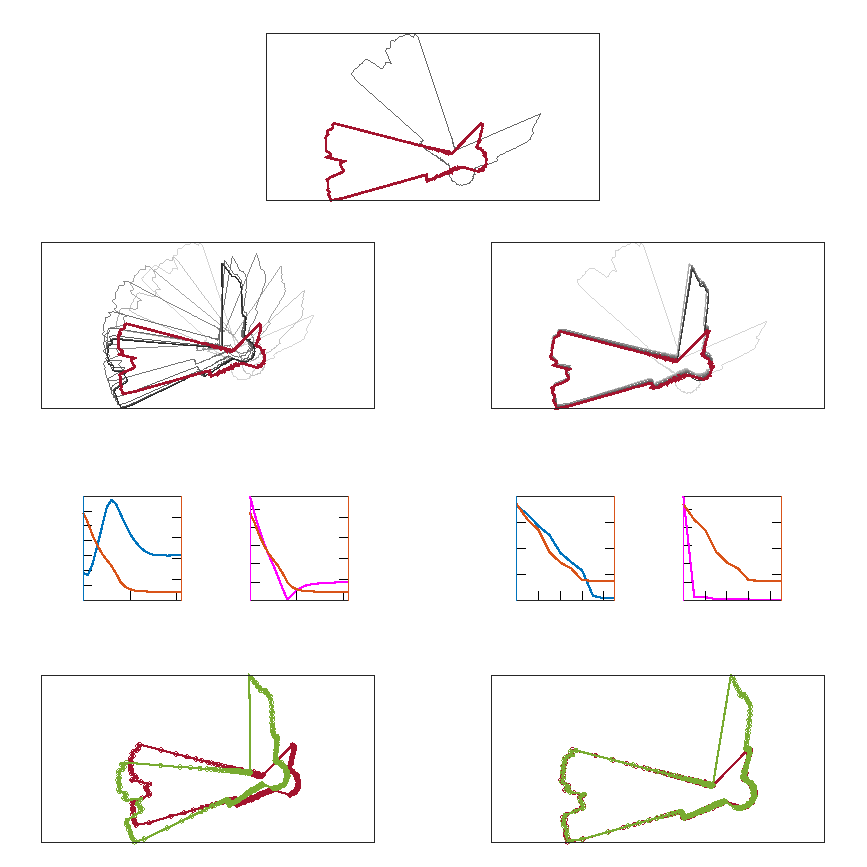
\includegraphics{./figures/parts/02/chapters/05/sections/04/fsm_vs_fgi}}%
    \gplfronttext
  \end{picture}%
\endgroup

  \vspace{0.5cm}
  \caption{\small Η εξέλιξη της διαδικασίας ευθυγράμμισης των δύο σαρώσεων του
           σχήματος της άνω σειράς μέσω του FastGICP (αριστερά) και του
           FSM (δεξιά). Οι δύο σαρώσεις διαταράσσονται από θόρυβο
           $\mathcal{N} \sim (0, 0.03^2)$ [m, m$^2$] και συλλαμβάνονται από
           στάσεις με διαφορά $\Delta = (0.35, 0.10, -\pi/3)$ [m,m,rad].
           Τα τελικά σφάλματα θέσης και προσανατολισμού του FastGICP είναι
           $0.61$ m και $0.173$ rad αντίστοιχα, ενώ του FSM
           $0.0098$ m και $0.0014$ rad}
  \label{fig:02_05_04:01}
\end{figure}


Στα σχήματα \ref{fig:02_05_04:02} και \ref{fig:02_05_04:03} απεικονίζεται η
χρησιμότητα της ευθυγράμμισης σαρώσεων: σε συνθήκες απουσίας χάρτη του
περιβάλλοντος μία μέθοδος ευθυγράμμισης σαρώσεων δρα ως παρατηρητής της στάσης
ενός ρομπότ (Παρατήρηση \ref{rem:sm_applications}). Στο πρόβλημα της
ευθυγράμμισης πραγματικών με εικονικές σαρώσεις (κεφ. \ref{part:02:chapter:04})
ο χάρτης δρα ως μέσο ανάδρασης λόγω της αντιστοιχίας του με το περιβάλλον και
του σταθερού συστήματος αναφοράς που ο ίδιος παρέχει---η απουσία του εδώ,
συνεπώς, αφαιρεί και τη δυνατότητα φραγής του σφάλματος εκτίμησης.\footnote{Η
ίδια απουσία σταθερού συστήματος αναφοράς βαραίνει ομοίως και την εκτίμηση της
στάσης του ρομπότ μέσω κωδικοποιητών.}

Στο σχήμα \ref{fig:02_05_04:02} παρατηρούμε πως σε ιδανικές συνθήκες ($\sigma_R
= 0.0$ m) οι PLICP και NDT εισάγουν οι ίδιες σφάλματα εκτίμησης---πιθανότατα
λόγω αποστάσεων θέσης και προσανατολισμού με μέτρο μεγαλύτερο από ότι μπορούν
να διορθώσουν με μεγαλύτερη ακρίβεια. Σε συνθήκες όπου ο αισθητήρας λαμβάνει
αραιότερα δείγματα στο χώρο αυτές οι αποστάσεις αυξάνουν, με αποτέλεσμα
αυξημένα σφάλματα. Σε αντίθεση ο FSM είναι ικανός να παρατηρήσει την τροχιά του
αισθητήρα με μεγαλύτερη ακρίβεια.

\begin{figure}[]\centering
  \begin{subfigure}{\linewidth}
    % GNUPLOT: LaTeX picture with Postscript
\begingroup
  \makeatletter
  \providecommand\color[2][]{%
    \GenericError{(gnuplot) \space\space\space\@spaces}{%
      Package color not loaded in conjunction with
      terminal option `colourtext'%
    }{See the gnuplot documentation for explanation.%
    }{Either use 'blacktext' in gnuplot or load the package
      color.sty in LaTeX.}%
    \renewcommand\color[2][]{}%
  }%
  \providecommand\includegraphics[2][]{%
    \GenericError{(gnuplot) \space\space\space\@spaces}{%
      Package graphicx or graphics not loaded%
    }{See the gnuplot documentation for explanation.%
    }{The gnuplot epslatex terminal needs graphicx.sty or graphics.sty.}%
    \renewcommand\includegraphics[2][]{}%
  }%
  \providecommand\rotatebox[2]{#2}%
  \@ifundefined{ifGPcolor}{%
    \newif\ifGPcolor
    \GPcolorfalse
  }{}%
  \@ifundefined{ifGPblacktext}{%
    \newif\ifGPblacktext
    \GPblacktexttrue
  }{}%
  % define a \g@addto@macro without @ in the name:
  \let\gplgaddtomacro\g@addto@macro
  % define empty templates for all commands taking text:
  \gdef\gplbacktext{}%
  \gdef\gplfronttext{}%
  \makeatother
  \ifGPblacktext
    % no textcolor at all
    \def\colorrgb#1{}%
    \def\colorgray#1{}%
  \else
    % gray or color?
    \ifGPcolor
      \def\colorrgb#1{\color[rgb]{#1}}%
      \def\colorgray#1{\color[gray]{#1}}%
      \expandafter\def\csname LTw\endcsname{\color{white}}%
      \expandafter\def\csname LTb\endcsname{\color{black}}%
      \expandafter\def\csname LTa\endcsname{\color{black}}%
      \expandafter\def\csname LT0\endcsname{\color[rgb]{1,0,0}}%
      \expandafter\def\csname LT1\endcsname{\color[rgb]{0,1,0}}%
      \expandafter\def\csname LT2\endcsname{\color[rgb]{0,0,1}}%
      \expandafter\def\csname LT3\endcsname{\color[rgb]{1,0,1}}%
      \expandafter\def\csname LT4\endcsname{\color[rgb]{0,1,1}}%
      \expandafter\def\csname LT5\endcsname{\color[rgb]{1,1,0}}%
      \expandafter\def\csname LT6\endcsname{\color[rgb]{0,0,0}}%
      \expandafter\def\csname LT7\endcsname{\color[rgb]{1,0.3,0}}%
      \expandafter\def\csname LT8\endcsname{\color[rgb]{0.5,0.5,0.5}}%
    \else
      % gray
      \def\colorrgb#1{\color{black}}%
      \def\colorgray#1{\color[gray]{#1}}%
      \expandafter\def\csname LTw\endcsname{\color{white}}%
      \expandafter\def\csname LTb\endcsname{\color{black}}%
      \expandafter\def\csname LTa\endcsname{\color{black}}%
      \expandafter\def\csname LT0\endcsname{\color{black}}%
      \expandafter\def\csname LT1\endcsname{\color{black}}%
      \expandafter\def\csname LT2\endcsname{\color{black}}%
      \expandafter\def\csname LT3\endcsname{\color{black}}%
      \expandafter\def\csname LT4\endcsname{\color{black}}%
      \expandafter\def\csname LT5\endcsname{\color{black}}%
      \expandafter\def\csname LT6\endcsname{\color{black}}%
      \expandafter\def\csname LT7\endcsname{\color{black}}%
      \expandafter\def\csname LT8\endcsname{\color{black}}%
    \fi
  \fi
    \setlength{\unitlength}{0.0500bp}%
    \ifx\gptboxheight\undefined%
      \newlength{\gptboxheight}%
      \newlength{\gptboxwidth}%
      \newsavebox{\gptboxtext}%
    \fi%
    \setlength{\fboxrule}{0.5pt}%
    \setlength{\fboxsep}{1pt}%
\begin{picture}(7000.00,7000.00)%
    \gplgaddtomacro\gplbacktext{%
      \colorrgb{0.15,0.15,0.15}%
      \put(600,2189){\makebox(0,0)[r]{\strut{}6}}%
      \colorrgb{0.15,0.15,0.15}%
      \put(600,2784){\makebox(0,0)[r]{\strut{}8}}%
      \colorrgb{0.15,0.15,0.15}%
      \put(600,3378){\makebox(0,0)[r]{\strut{}10}}%
      \colorrgb{0.15,0.15,0.15}%
      \put(600,3973){\makebox(0,0)[r]{\strut{}12}}%
      \colorrgb{0.15,0.15,0.15}%
      \put(600,4567){\makebox(0,0)[r]{\strut{}14}}%
      \colorrgb{0.15,0.15,0.15}%
      \put(600,5162){\makebox(0,0)[r]{\strut{}16}}%
      \colorrgb{0.00,0.00,0.00}%
      \put(940,1880){\makebox(0,0){\strut{}-2}}%
      \colorrgb{0.00,0.00,0.00}%
      \put(1535,1880){\makebox(0,0){\strut{}0}}%
      \colorrgb{0.00,0.00,0.00}%
      \put(2129,1880){\makebox(0,0){\strut{}2}}%
      \colorrgb{0.00,0.00,0.00}%
      \put(2724,1880){\makebox(0,0){\strut{}4}}%
      \colorrgb{0.00,0.00,0.00}%
      \put(3318,1880){\makebox(0,0){\strut{}6}}%
    }%
    \gplgaddtomacro\gplfronttext{%
    }%
    \gplgaddtomacro\gplbacktext{%
      \colorrgb{0.00,0.00,0.00}%
      \put(3950,1880){\makebox(0,0){\strut{}-2}}%
      \colorrgb{0.00,0.00,0.00}%
      \put(4544,1880){\makebox(0,0){\strut{}0}}%
      \colorrgb{0.00,0.00,0.00}%
      \put(5139,1880){\makebox(0,0){\strut{}2}}%
      \colorrgb{0.00,0.00,0.00}%
      \put(5733,1880){\makebox(0,0){\strut{}4}}%
      \colorrgb{0.00,0.00,0.00}%
      \put(6327,1880){\makebox(0,0){\strut{}6}}%
    }%
    \gplgaddtomacro\gplfronttext{%
    }%
    \gplbacktext
    \put(0,0){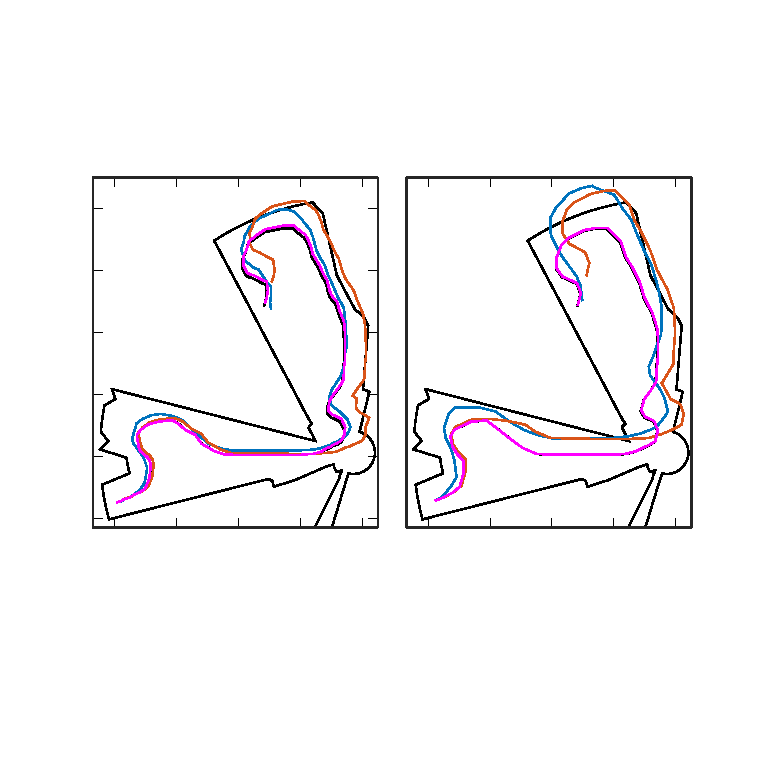
\includegraphics{/media/li9i/var/elements/PhD/fourier_scan_matcher/scripts_phd/characterisation/laser_odometry/odom_test_5_vs_6_sr_000}}%
    \gplfronttext
  \end{picture}%
\endgroup

  \end{subfigure}\\ \vspace{-5cm}
  \begin{subfigure}{\linewidth}
    % GNUPLOT: LaTeX picture with Postscript
\begingroup
  \makeatletter
  \providecommand\color[2][]{%
    \GenericError{(gnuplot) \space\space\space\@spaces}{%
      Package color not loaded in conjunction with
      terminal option `colourtext'%
    }{See the gnuplot documentation for explanation.%
    }{Either use 'blacktext' in gnuplot or load the package
      color.sty in LaTeX.}%
    \renewcommand\color[2][]{}%
  }%
  \providecommand\includegraphics[2][]{%
    \GenericError{(gnuplot) \space\space\space\@spaces}{%
      Package graphicx or graphics not loaded%
    }{See the gnuplot documentation for explanation.%
    }{The gnuplot epslatex terminal needs graphicx.sty or graphics.sty.}%
    \renewcommand\includegraphics[2][]{}%
  }%
  \providecommand\rotatebox[2]{#2}%
  \@ifundefined{ifGPcolor}{%
    \newif\ifGPcolor
    \GPcolorfalse
  }{}%
  \@ifundefined{ifGPblacktext}{%
    \newif\ifGPblacktext
    \GPblacktexttrue
  }{}%
  % define a \g@addto@macro without @ in the name:
  \let\gplgaddtomacro\g@addto@macro
  % define empty templates for all commands taking text:
  \gdef\gplfronttext{}%
  \gdef\gplfronttext{}%
  \makeatother
  \ifGPblacktext
    % no textcolor at all
    \def\colorrgb#1{}%
    \def\colorgray#1{}%
  \else
    % gray or color?
    \ifGPcolor
      \def\colorrgb#1{\color[rgb]{#1}}%
      \def\colorgray#1{\color[gray]{#1}}%
      \expandafter\def\csname LTw\endcsname{\color{white}}%
      \expandafter\def\csname LTb\endcsname{\color{black}}%
      \expandafter\def\csname LTa\endcsname{\color{black}}%
      \expandafter\def\csname LT0\endcsname{\color[rgb]{1,0,0}}%
      \expandafter\def\csname LT1\endcsname{\color[rgb]{0,1,0}}%
      \expandafter\def\csname LT2\endcsname{\color[rgb]{0,0,1}}%
      \expandafter\def\csname LT3\endcsname{\color[rgb]{1,0,1}}%
      \expandafter\def\csname LT4\endcsname{\color[rgb]{0,1,1}}%
      \expandafter\def\csname LT5\endcsname{\color[rgb]{1,1,0}}%
      \expandafter\def\csname LT6\endcsname{\color[rgb]{0,0,0}}%
      \expandafter\def\csname LT7\endcsname{\color[rgb]{1,0.3,0}}%
      \expandafter\def\csname LT8\endcsname{\color[rgb]{0.5,0.5,0.5}}%
    \else
      % gray
      \def\colorrgb#1{\color{black}}%
      \def\colorgray#1{\color[gray]{#1}}%
      \expandafter\def\csname LTw\endcsname{\color{white}}%
      \expandafter\def\csname LTb\endcsname{\color{black}}%
      \expandafter\def\csname LTa\endcsname{\color{black}}%
      \expandafter\def\csname LT0\endcsname{\color{black}}%
      \expandafter\def\csname LT1\endcsname{\color{black}}%
      \expandafter\def\csname LT2\endcsname{\color{black}}%
      \expandafter\def\csname LT3\endcsname{\color{black}}%
      \expandafter\def\csname LT4\endcsname{\color{black}}%
      \expandafter\def\csname LT5\endcsname{\color{black}}%
      \expandafter\def\csname LT6\endcsname{\color{black}}%
      \expandafter\def\csname LT7\endcsname{\color{black}}%
      \expandafter\def\csname LT8\endcsname{\color{black}}%
    \fi
  \fi
    \setlength{\unitlength}{0.02500bp}%
    \ifx\gptboxheight\undefined%
      \newlength{\gptboxheight}%
      \newlength{\gptboxwidth}%
      \newsavebox{\gptboxtext}%
    \fi%
    \setlength{\fboxrule}{0.5pt}%
    \setlength{\fboxsep}{1pt}%
\hspace{1cm}
\begin{picture}(7000.00,7000.00)%
    \gplgaddtomacro\gplfronttext{%
      \colorrgb{0.15,0.15,0.15}%
      \put(600,2189){\makebox(0,0)[r]{\strut{}\scriptsize $6.0$}}%
      \colorrgb{0.15,0.15,0.15}%
      \put(600,2784){\makebox(0,0)[r]{\strut{}\scriptsize $8.0$}}%
      \colorrgb{0.15,0.15,0.15}%
      \put(600,3378){\makebox(0,0)[r]{\strut{}\scriptsize $10.0$}}%
      \colorrgb{0.15,0.15,0.15}%
      \put(600,3973){\makebox(0,0)[r]{\strut{}\scriptsize $12.0$}}%
      \colorrgb{0.15,0.15,0.15}%
      \put(600,4567){\makebox(0,0)[r]{\strut{}\scriptsize $14.0$}}%
      \colorrgb{0.15,0.15,0.15}%
      \put(600,5162){\makebox(0,0)[r]{\strut{}\scriptsize $16.0$}}%
      \colorrgb{0.00,0.00,0.00}%
      \put(940,1880){\makebox(0,0){\strut{} \scriptsize $-2.0$}}%
      \colorrgb{0.00,0.00,0.00}%
      %\put(1535,1880){\makebox(0,0){\strut{}\scriptsize $0.0$}}%
      \colorrgb{0.00,0.00,0.00}%
      \put(2129,1880){\makebox(0,0){\strut{}\scriptsize $2.0$}}%
      \colorrgb{0.00,0.00,0.00}%
      \put(2724,1880){\makebox(0,0){\strut{}\scriptsize $4.0$}}%
      \colorrgb{0.00,0.00,0.00}%
      \put(3318,1880){\makebox(0,0){\strut{}\scriptsize $6.0$}}%

      \put(-800,4900){\rotatebox{90}{\makebox(0,0)[r]{\strut{}$\sigma_R = 0.05$ m}}}%
      \put(1800,1504){\makebox(0,0){\strut{} \scriptsize Συχνές μετρήσεις}}
      \put(5100,1504){\makebox(0,0){\strut{} \scriptsize Σποραδικές μετρήσεις}}
    }%
    \gplgaddtomacro\gplfronttext{%
    }%
    \gplgaddtomacro\gplfronttext{%
      \colorrgb{0.00,0.00,0.00}%
      \put(3950,1880){\makebox(0,0){\strut{}\scriptsize $-2.0$}}%
      \colorrgb{0.00,0.00,0.00}%
      %\put(4544,1880){\makebox(0,0){\strut{}\scriptsize $0.0$}}%
      \colorrgb{0.00,0.00,0.00}%
      \put(5139,1880){\makebox(0,0){\strut{}\scriptsize $2.0$}}%
      \colorrgb{0.00,0.00,0.00}%
      \put(5733,1880){\makebox(0,0){\strut{}\scriptsize $4.0$}}%
      \colorrgb{0.00,0.00,0.00}%
      \put(6327,1880){\makebox(0,0){\strut{}\scriptsize $6.0$}}%
    }%
    \gplgaddtomacro\gplfronttext{%
    }%
    \put(0,0){\animategraphics[autoplay,scale=0.5]{10}{./figures/slides/ch7/odom/sim/laser_odometry/imgs/odom_test_5_vs_6_sr_005_}{1}{110}}%
    \gplfronttext
  \end{picture}%
\endgroup

  \end{subfigure}
  \vspace{-2cm}
  \caption{\small Η ευθυγράμμιση σαρώσεων ως μέσο παρατήρησης της τροχιάς του
           αισθητήρα, ή αλλιώς ως ``laser odometry": το ρομπότ κινείται από
           την κάτω αριστερά περιοχή του περιβάλλοντος προς την άνω δεξιά,
           συλλαμβάνοντας μετρήσεις καθ' οδόν. Οι χρωματισμένες γραμμές
           απεικονίζουν τις εκτιμώμενες τροχιές του αισθητήρα από κάθε μέθοδο.
           Στα διαγράμματα της αριστερής πλευράς ο αισθητήρας αποστάσεων
           συλλέγει συχνότερα μετρήσεις από ότι στα διαγράμματα της δεξιάς
           πλευράς, με αποτέλεσμα πυκνότερες μετρήσεις στο χώρο, συλληφθείσες
           από στάσεις με μικρότερη απόσταση θέσεων, και συνεπώς με
           μεγαλύτερη αλληλοεπικάλυψη. Στα διαγράμματα της άνω σειράς ο
           αισθητήρας αναφέρει τέλειες μετρήσεις, ενώ στα διαγράμματα της κάτω
           σειράς μετρήσεις στις οποίες επιδρούν διαταραχές
           $\mathcal{N}\sim(0,0.05^2)$ [m,m$^2$]}
  \label{fig:02_05_04:02}
\end{figure}

Στο σχήμα \ref{fig:02_05_04:03} απεικονίζεται η εκτιμώμενη από τις μεθόδους
PLICP, NDT, FastGICP, FastVGICP, και FSM τροχιά ενός πανοραμικού φυσικού
αισθητήρα YDLIDAR TG30, $2019$ ακτίνων, στο περιβάλλον του οποίου ο χάρτης
απεικονίζει με άσπρο χρώμα τον ελεύθερό του χώρο.\footnote{Η εξαγωγή του χάρτη
του περιβάλλοντος και η συλλογή μετρήσεων από τον αισθητήρα για τους σκοπούς
του πειράματος διεξήχθησαν σε διαφορετικούς χρόνους και μέσω διαφορετικών
αισθητήρων, ενώ το ύψος των αισθητήρων από το δάπεδο ήταν διαφορετικό (στην
πρώτη περίπτωση ο αισθητήρας τοποθετήθηκε $\simeq 0.60$ m από το έδαφος, ενώ
στην δεύτερη $\simeq 1.85$ m από το έδαφος). Στην πρώτη περίπτωση η πρόσβαση
στον χώρο $\otimes_5$ ήταν αποκεκλεισμένη, ενώ στη δεύτερη ελεύθερη.  Ο εν λόγω
χώρος είναι ορθογώνιος και αποτελείται από ένα επίσης ορθογώνιο εμπόδιο,
τοποθετημένο στη νότια πλευρά του και κάθετα στον οριζόντιο
άξονα.}\textsuperscript{,}\footnote{Κατά τη συλλογή των μετρήσεων ήταν
διαθέσιμος μόνο ο αισθητήρας αποστάσεων, και συνεπώς οι εκτιμητέες στάσεις δεν
έχουν γνωστό σύστημα αναφοράς. Κατά συνέπεια ο χάρτης επικαλύφθηκε με τις
εκτιμητέες τροχιές με ευρηστικό τρόπο για κάθε τροχιά, και συγκεκριμένα ώστε οι
τροχιές να είναι όσο το δυνατό ευθυγραμμισμένες με τη δίοδο από τις θύρες των
χώρων.} Στις μετρήσεις του αισθητήρα επιδρούν διαταραχές αγνώστης κατανομής και
αγνώστου μεγίστου μέτρου, αλλά γνωστής μέσης τιμής ανά ζώνη αναφερόμενης
απόστασης από κάθε ακτίνα του. Η μέση τιμή των διαταραχών και το συνολικό
ποσοστό των αποστάσεων που καταγράφηκαν στο συγκεκριμένο πείραμα αναφέρονται
κατά ζώνη στον πίνακα \ref{tbl:02:05_04:tg30}.  Σύμφωνα με τα πειραματικά
αποτελέσματα του σχήματος \ref{fig:02_05_04:03} και τα αποτελέσματα που
προέκυψαν μέσω προσομοιώσεων---τα οποία απεικονίζονται στο σχήμα
\ref{fig:02_05_04:02}---οι δύο ιεραρχίες των τριών μεθόδων με βάση τα σφάλματα
εκτίμησης τους είναι κατά κύριο λόγο συνεπείς μεταξύ τους.  Επιπρόσθετα, μόνο
οι τροχιές των μεθόδων PLICP, FastGICP, και FSM προσομοιάζουν στην πραγματική
τροχιά του αισθητήρα (---για την οποία είναι γνωστή μόνο η τοπολογική τροχία
της, η οποία έχει αφετηρία το χώρο $\otimes_0$ και τέρμα στη γειτονιά της
συντεταγμένης $(16.0, 17.0)$).


\begin{table}[h]\centering \vspace{0.5cm}
  \begin{tabular}{rcc}
    Απόσταση $d$ [mm]   & Μέσο σφάλμα [mm]    & Ποσοστό αποστάσεων $\leq d$ σχ. \ref{fig:02_05_04:03} \\ \toprule
    $50$-$5000$         & $\leq \pm 60$       & $89.06\%$  \\
    $5000$-$20000$      & $\leq \pm 40$       & $10.94\%$  \\
    $20000$-$30000$     & $\leq \pm 100$      & $0.0\%$    \\  \bottomrule
  \end{tabular}
  \caption{\small Το μέσο σφάλμα των μετρήσεων του αισθητήρα YDLIDAR TG30
           εξαρτάται από την ίδια την ανιχνευόμενη απόσταση $d$. Η τρίτη στήλη
           παρουσιάζει τα ποσοστά των μετρήσεων του αισθητήρα ανά ζώνη της
           πρώτης στήλης καθώς αυτός κινήθηκε στο περιβάλλον του οποίου ο
           χάρτης απεικονίζεται στο σχήμα \ref{fig:02_05_04:03}. Ο αισθητήρας
           ανήκει στην κατηγορία των πανοραμικών αισθητήρων απόστασης
           δισδιάστατων μετρήσεων με ελκυστική τιμή αλλά υψηλά επίπεδα
           θορύβου. Πηγή: \url{https://www.ydlidar.com/Public/upload/files/2022-03-22/YDLIDAR\%20TG30\%20Data\%20Sheet\%20V1.4(211230).pdf}, εν. 2.2}
  \label{tbl:02:05_04:tg30}
\end{table}

\begin{figure}[]\centering
  \definecolor{plicp}{rgb}{0.00000   0.44700   0.74100}
\definecolor{ndt}{rgb}{0.85000   0.32500   0.09800}
\definecolor{fgi}{rgb}{0.9290 0.6940 0.1250}
\definecolor{fvg}{rgb}{0.4940 0.1840 0.5560}
\definecolor{fmt}{rgb}{1.00000   0.00000   1.00000}
\definecolor{gg}{RGB}{156 156 156}

% GNUPLOT: LaTeX picture with Postscript
\begingroup
  \makeatletter
  \providecommand\color[2][]{%
    \GenericError{(gnuplot) \space\space\space\@spaces}{%
      Package color not loaded in conjunction with
      terminal option `colourtext'%
    }{See the gnuplot documentation for explanation.%
    }{Either use 'blacktext' in gnuplot or load the package
      color.sty in LaTeX.}%
    \renewcommand\color[2][]{}%
  }%
  \providecommand\includegraphics[2][]{%
    \GenericError{(gnuplot) \space\space\space\@spaces}{%
      Package graphicx or graphics not loaded%
    }{See the gnuplot documentation for explanation.%
    }{The gnuplot epslatex terminal needs graphicx.sty or graphics.sty.}%
    \renewcommand\includegraphics[2][]{}%
  }%
  \providecommand\rotatebox[2]{#2}%
  \@ifundefined{ifGPcolor}{%
    \newif\ifGPcolor
    \GPcolorfalse
  }{}%
  \@ifundefined{ifGPblacktext}{%
    \newif\ifGPblacktext
    \GPblacktexttrue
  }{}%
  % define a \g@addto@macro without @ in the name:
  \let\gplgaddtomacro\g@addto@macro
  % define empty templates for all commands taking text:
  \gdef\gplfronttext{}%
  \gdef\gplfronttext{}%
  \makeatother
  \ifGPblacktext
    % no textcolor at all
    \def\colorrgb#1{}%
    \def\colorgray#1{}%
  \else
    % gray or color?
    \ifGPcolor
      \def\colorrgb#1{\color[rgb]{#1}}%
      \def\colorgray#1{\color[gray]{#1}}%
      \expandafter\def\csname LTw\endcsname{\color{white}}%
      \expandafter\def\csname LTb\endcsname{\color{black}}%
      \expandafter\def\csname LTa\endcsname{\color{black}}%
      \expandafter\def\csname LT0\endcsname{\color[rgb]{1,0,0}}%
      \expandafter\def\csname LT1\endcsname{\color[rgb]{0,1,0}}%
      \expandafter\def\csname LT2\endcsname{\color[rgb]{0,0,1}}%
      \expandafter\def\csname LT3\endcsname{\color[rgb]{1,0,1}}%
      \expandafter\def\csname LT4\endcsname{\color[rgb]{0,1,1}}%
      \expandafter\def\csname LT5\endcsname{\color[rgb]{1,1,0}}%
      \expandafter\def\csname LT6\endcsname{\color[rgb]{0,0,0}}%
      \expandafter\def\csname LT7\endcsname{\color[rgb]{1,0.3,0}}%
      \expandafter\def\csname LT8\endcsname{\color[rgb]{0.5,0.5,0.5}}%
    \else
      % gray
      \def\colorrgb#1{\color{black}}%
      \def\colorgray#1{\color[gray]{#1}}%
      \expandafter\def\csname LTw\endcsname{\color{white}}%
      \expandafter\def\csname LTb\endcsname{\color{black}}%
      \expandafter\def\csname LTa\endcsname{\color{black}}%
      \expandafter\def\csname LT0\endcsname{\color{black}}%
      \expandafter\def\csname LT1\endcsname{\color{black}}%
      \expandafter\def\csname LT2\endcsname{\color{black}}%
      \expandafter\def\csname LT3\endcsname{\color{black}}%
      \expandafter\def\csname LT4\endcsname{\color{black}}%
      \expandafter\def\csname LT5\endcsname{\color{black}}%
      \expandafter\def\csname LT6\endcsname{\color{black}}%
      \expandafter\def\csname LT7\endcsname{\color{black}}%
      \expandafter\def\csname LT8\endcsname{\color{black}}%
    \fi
  \fi
    \setlength{\unitlength}{0.0500bp}%
    \ifx\gptboxheight\undefined%
      \newlength{\gptboxheight}%
      \newlength{\gptboxwidth}%
      \newsavebox{\gptboxtext}%
    \fi%
    \setlength{\fboxrule}{0.5pt}%
    \setlength{\fboxsep}{1pt}%
\begin{picture}(8000.00,4000.00)%
    \gplgaddtomacro\gplfronttext{%
      \put(1000,3900){\makebox(0,0){\strut{}{\color{plicp}{\rule[0.6mm]{0.5cm}{0.5mm}}} PLICP}}
      \put(2500,3900){\makebox(0,0){\strut{}{\color{ndt}{\rule[0.6mm]{0.5cm}{0.5mm}}} NDT}}
      \put(4000,3900){\makebox(0,0){\strut{}{\color{fgi}{\rule[0.6mm]{0.5cm}{0.5mm}}} GICP}}
      \put(5500,3900){\makebox(0,0){\strut{}{\color{fvg}{\rule[0.6mm]{0.5cm}{0.5mm}}} VGICP}}
      \put(7000,3900){\makebox(0,0){\strut{}{\color{fmt}{\rule[0.6mm]{0.5cm}{0.5mm}}} \texttt{fsm}}}
    }%
    \gplgaddtomacro\gplfronttext{%
      \colorrgb{0.15,0.15,0.15}%
      \put(953,3206){\makebox(0,0)[r]{\strut{}$21.0$}}%
      \colorrgb{0.15,0.15,0.15}%
      \put(953,2466){\makebox(0,0)[r]{\strut{}$19.0$}}%
      \colorrgb{0.15,0.15,0.15}%
      \put(953,1726){\makebox(0,0)[r]{\strut{}$17.0$}}%
      \colorrgb{0.15,0.15,0.15}%
      \put(953,986){\makebox(0,0)[r]{\strut{}$15.0$}}%
      \colorrgb{0.15,0.15,0.15}%
      \put(1455,3326){\makebox(0,0){\strut{}$12.0$}}%
      \colorrgb{0.15,0.15,0.15}%
      \put(2935,3326){\makebox(0,0){\strut{}$16.0$}}%
      \colorrgb{0.15,0.15,0.15}%
      \put(4416,3326){\makebox(0,0){\strut{}$20.0$}}%
      \colorrgb{0.15,0.15,0.15}%
      \put(5896,3326){\makebox(0,0){\strut{}$24.0$}}%
      \colorrgb{0.15,0.15,0.15}%
      \put(7376,3326){\makebox(0,0){\strut{}$28.0$}}%
    }%
    \put(0,0){\animategraphics[autoplay,loop]{0.5}{./figures/slides/ch7/odom/real/odom_test_ag10/odom_test_}{1}{10}}%
    \gplfronttext
  \end{picture}%
\endgroup

  \vspace{0.25cm}
  \caption{\small Εκτιμήσεις της πραγματικής τροχιάς του φυσικού αισθητήρα
           YDLIDAR TG30 από τις μεθόδους που είναι ικανές για εκτέλεση σε
           πραγματικό χρόνο καθώς αυτός κινείται με τροχιά $\otimes_0
           \Rightarrow \otimes_1 \Rightarrow \otimes_2 \Rightarrow \otimes_3
           \Rightarrow \otimes_1 \Rightarrow \otimes_4 \Rightarrow \otimes_5
           \rightarrow \otimes_0$. Η πραγματική τροχιά είναι εν γένει λεία.
           Ο χώρος με κέντρο το σύμβολο $\otimes_5$ είναι κατειλλημμένος.
           Καθώς στο πρόβλημα της παραγωγής οδομετρίας από μετρήσεις αποστάσεων
           το τελικό σφάλμα θέσης είναι μη φραγμένο και συσσωρευόμενο, ένας
           επιπρόσθετος τρόπος αξιολόγησης της επίδοσης των μεθόδων συνίσταται
           στον υπολογισμό του σφάλματος της τελευταίας τους εκτίμησης---η
           τελική πραγματική θέση του αισθητήρα σε αυτήν την περίπτωση
           είναι στη γειτονιά της συντεταγμένης $(16.0,17.0)$ m}
  \label{fig:02_05_04:03}
\end{figure}


Ως προς τους περιορισμούς της απόκρισης των μεθόδων ευθυγράμμισης σαρώσεων, οι
κύριοι από αυτούς είναι οι ίδιοι με αυτούς των προσθετικών μεθόδων
ευθυγράμμισης πραγματικών με εικονικές σαρώσεις. Αυτοί αφορούν στα αμετάβλητα
χαρακτηριστικά μεγέθη του φυσικού αισθητήρα σαρώσεων, τα οποία είναι δυο. Το
πρώτο είναι το μέγεθος των διαταραχών που επιδρούν στις μετρήσεις του, την
απόκριση επί του οποίου εξετάσαμε για διάφορες τιμές στην ενότητα
\ref{section:02_05_03}. Το δεύτερο είναι το βεληνεκές του αισθητήρα, δηλαδή η
μέγιστη απόσταση μέχρι την οποία μπορεί να ανιχνεύσει την παρουσία
αντικειμένων.

Στην άνω σειρά του σχήματος \ref{fig:02_05_04:04} εμφανίζονται με λευκό χρώμα
δύο διαφορετικά περιβάλλοντα, μέσα στα οποία τοποθετείται ένας αισθητήρας στις
θέσεις που σημειώνονται με κουκκίδες βαθύ μπλε χρώματος. Οι θέσεις αυτές είναι
τα κέντρα των ομόκεντρων κύκλων που εμφανίζονται στην ίδια σειρά. Η πειραματική
διάταξη που ακολουθεί στοχεύει στην καταγραφή της απόκρισης των μεθόδων
PLICP και FSM σε πειράματα όπου το βεληνεκές του αισθητήρα
μεταβάλλεται έτσι ώστε οι μετρήσεις του να περιλαμβάνουν όλα τα εμπόδια του
περιβάλλοντος, μειούμενο μέχρι που να μην περιλαμβάνουν κανένα. Το βεληνεκές
του αισθητήρα είναι η ακτίνα των κύκλων της πρώτης σειράς του σχήματος, και το
χρώμα αυτών αναπαριστά το ποσοστό των ακτίνων που φέρουν χωρική πληροφορία,
βάσει της χρωματικής λωρίδας που παρουσιάζεται στη δεύτερη σειρά. Στις δύο
τελευταίες σειρές παρατίθενται οι μέσοι όροι των σφαλμάτων εκτίμησης
προσανατολισμού και θέσης σε δέκα επαναλήψεις, για κάθε μέθοδο και περιβάλλον,
για $\sigma_R = 0.05$ m. Η δεύτερη στάση του αισθητήρα παράγεται τυχαία για
κάθε πείραμα μέσω διαταραχής των αντίστοιχων συνιστωσών της πρώτης στάσης του
αισθητήρα με ποσότητες που εξάγονται από τις ομοιόμορφες κατανομές
$U_{xy}(-\overline{\delta}_{xy},+\overline{\delta}_{xy})$ m και
$U_{\theta}(-\overline{\delta}_{\theta},+\overline{\delta}_{\theta})$ rad.
Συγκεκριμένα δοκιμάζονται δύο διαμορφώσεις αρχικών συνθηκών. H πρώτη
συμβολίζεται με $\Delta_\alpha$, για την οποία
$(\overline{\delta}_{xy}, \overline{\delta}_{\theta}) = (0.05,0.174)$ [m,rad].
Η δεύτερη συμβολίζεται με $\Delta_\beta$, για την οποία
$(\overline{\delta}_{xy},\overline{\delta}_{\theta}) = (0.20,\pi/4)$ [m,rad].

\begin{figure}[]\centering
  \definecolor{aa}{rgb}{0.00000   0.44700   0.74100}
\definecolor{ac}{rgb}{1.00000   0.00000   1.00000}

% GNUPLOT: LaTeX picture with Postscript
\begingroup
  \makeatletter
  \providecommand\color[2][]{%
    \GenericError{(gnuplot) \space\space\space\@spaces}{%
      Package color not loaded in conjunction with
      terminal option `colourtext'%
    }{See the gnuplot documentation for explanation.%
    }{Either use 'blacktext' in gnuplot or load the package
      color.sty in LaTeX.}%
    \renewcommand\color[2][]{}%
  }%
  \providecommand\includegraphics[2][]{%
    \GenericError{(gnuplot) \space\space\space\@spaces}{%
      Package graphicx or graphics not loaded%
    }{See the gnuplot documentation for explanation.%
    }{The gnuplot epslatex terminal needs graphicx.sty or graphics.sty.}%
    \renewcommand\includegraphics[2][]{}%
  }%
  \providecommand\rotatebox[2]{#2}%
  \@ifundefined{ifGPcolor}{%
    \newif\ifGPcolor
    \GPcolorfalse
  }{}%
  \@ifundefined{ifGPblacktext}{%
    \newif\ifGPblacktext
    \GPblacktexttrue
  }{}%
  % define a \g@addto@macro without @ in the name:
  \let\gplgaddtomacro\g@addto@macro
  % define empty templates for all commands taking text:
  \gdef\gplfronttext{}%
  \gdef\gplfronttext{}%
  \makeatother
  \ifGPblacktext
    % no textcolor at all
    \def\colorrgb#1{}%
    \def\colorgray#1{}%
  \else
    % gray or color?
    \ifGPcolor
      \def\colorrgb#1{\color[rgb]{#1}}%
      \def\colorgray#1{\color[gray]{#1}}%
      \expandafter\def\csname LTw\endcsname{\color{white}}%
      \expandafter\def\csname LTb\endcsname{\color{black}}%
      \expandafter\def\csname LTa\endcsname{\color{black}}%
      \expandafter\def\csname LT0\endcsname{\color[rgb]{1,0,0}}%
      \expandafter\def\csname LT1\endcsname{\color[rgb]{0,1,0}}%
      \expandafter\def\csname LT2\endcsname{\color[rgb]{0,0,1}}%
      \expandafter\def\csname LT3\endcsname{\color[rgb]{1,0,1}}%
      \expandafter\def\csname LT4\endcsname{\color[rgb]{0,1,1}}%
      \expandafter\def\csname LT5\endcsname{\color[rgb]{1,1,0}}%
      \expandafter\def\csname LT6\endcsname{\color[rgb]{0,0,0}}%
      \expandafter\def\csname LT7\endcsname{\color[rgb]{1,0.3,0}}%
      \expandafter\def\csname LT8\endcsname{\color[rgb]{0.5,0.5,0.5}}%
    \else
      % gray
      \def\colorrgb#1{\color{black}}%
      \def\colorgray#1{\color[gray]{#1}}%
      \expandafter\def\csname LTw\endcsname{\color{white}}%
      \expandafter\def\csname LTb\endcsname{\color{black}}%
      \expandafter\def\csname LTa\endcsname{\color{black}}%
      \expandafter\def\csname LT0\endcsname{\color{black}}%
      \expandafter\def\csname LT1\endcsname{\color{black}}%
      \expandafter\def\csname LT2\endcsname{\color{black}}%
      \expandafter\def\csname LT3\endcsname{\color{black}}%
      \expandafter\def\csname LT4\endcsname{\color{black}}%
      \expandafter\def\csname LT5\endcsname{\color{black}}%
      \expandafter\def\csname LT6\endcsname{\color{black}}%
      \expandafter\def\csname LT7\endcsname{\color{black}}%
      \expandafter\def\csname LT8\endcsname{\color{black}}%
    \fi
  \fi
    \setlength{\unitlength}{0.0500bp}%
    \ifx\gptboxheight\undefined%
      \newlength{\gptboxheight}%
      \newlength{\gptboxwidth}%
      \newsavebox{\gptboxtext}%
    \fi%
    \setlength{\fboxrule}{0.5pt}%
    \setlength{\fboxsep}{1pt}%
\begin{picture}(8000.00,10000.00)%
    \gplgaddtomacro\gplfronttext{%
    }%
    \gplgaddtomacro\gplfronttext{%
    }%
    \gplgaddtomacro\gplfronttext{%
    }%
    \gplgaddtomacro\gplfronttext{%
    }%
    \gplgaddtomacro\gplfronttext{%
    }%
    \gplgaddtomacro\gplfronttext{%
      \colorrgb{0.00,0.00,0.00}%
      \put(3999,7219){\makebox(0,0){\strut{}Χρωματική αναπαράσταση ποσοστού ακτίνων εντός μέγιστου εύρους αισθητήρα}}%
    }%
    \gplgaddtomacro\gplfronttext{%
    }%
    \gplgaddtomacro\gplfronttext{%
      \colorrgb{0.15,0.15,0.15}%
      \put(1040,6580){\makebox(0,0){\strut{}\small $0\%$}}%
      \colorrgb{0.15,0.15,0.15}%
      \put(2280,6580){\makebox(0,0){\strut{}\small $20\%$}}%
      \colorrgb{0.15,0.15,0.15}%
      \put(3520,6580){\makebox(0,0){\strut{}\small $40\%$}}%
      \colorrgb{0.15,0.15,0.15}%
      \put(4759,6580){\makebox(0,0){\strut{}\small $60\%$}}%
      \colorrgb{0.15,0.15,0.15}%
      \put(5999,6580){\makebox(0,0){\strut{}\small $80\%$}}%
      \colorrgb{0.15,0.15,0.15}%
      \put(7239,6580){\makebox(0,0){\strut{}\small $100\%$}}%
    }%
    \gplgaddtomacro\gplfronttext{%
      \colorrgb{0.15,0.15,0.15}%
      \put(768,4000){\makebox(0,0)[r]{\strut{}\scriptsize $0.0$}}%
      \colorrgb{0.15,0.15,0.15}%
      \put(768,4374){\makebox(0,0)[r]{\strut{}\scriptsize $0.035$}}%
      \colorrgb{0.15,0.15,0.15}%
      \put(768,4747){\makebox(0,0)[r]{\strut{}\scriptsize $0.070$}}%
      \colorrgb{0.15,0.15,0.15}%
      \put(768,5121){\makebox(0,0)[r]{\strut{}\scriptsize $0.105$}}%
      \colorrgb{0.15,0.15,0.15}%
      \put(768,5495){\makebox(0,0)[r]{\strut{}\scriptsize $0.140$}}%
      \colorrgb{0.15,0.15,0.15}%
      \put(800,3780){\makebox(0,0){\strut{}}}%
      \colorrgb{0.15,0.15,0.15}%
      \put(1040,3780){\makebox(0,0){\strut{}}}%
      \colorrgb{0.15,0.15,0.15}%
      \put(1280,3780){\makebox(0,0){\strut{}}}%
      \colorrgb{0.15,0.15,0.15}%
      \put(1519,3780){\makebox(0,0){\strut{}}}%
      \colorrgb{0.15,0.15,0.15}%
      \put(1759,3780){\makebox(0,0){\strut{}}}%
      \colorrgb{0.15,0.15,0.15}%
      \put(1999,3780){\makebox(0,0){\strut{}}}%
    }%
    \gplgaddtomacro\gplfronttext{%
      \colorrgb{0.15,0.15,0.15}%
      \put(-200,4749){\rotatebox{90}{\makebox(0,0){\strut{}$e_{\theta}$ [rad]}}}%
      \colorrgb{0.00,0.00,0.00}%
      \put(1399,5719){\makebox(0,0){\strut{}$\Delta_{\alpha}$}}%
    }%
    \gplgaddtomacro\gplfronttext{%
      \colorrgb{0.15,0.15,0.15}%
      \put(2448,4000){\makebox(0,0)[r]{\strut{}\scriptsize $0.0$}}%
      \colorrgb{0.15,0.15,0.15}%
      \put(2448,4503){\makebox(0,0)[r]{\strut{}\scriptsize $0.17$}}%
      \colorrgb{0.15,0.15,0.15}%
      \put(2448,5006){\makebox(0,0)[r]{\strut{}\scriptsize $0.35$}}%
      \colorrgb{0.15,0.15,0.15}%
      \put(2480,3780){\makebox(0,0){\strut{}}}%
      \colorrgb{0.15,0.15,0.15}%
      \put(2720,3780){\makebox(0,0){\strut{}}}%
      \colorrgb{0.15,0.15,0.15}%
      \put(2960,3780){\makebox(0,0){\strut{}}}%
      \colorrgb{0.15,0.15,0.15}%
      \put(3199,3780){\makebox(0,0){\strut{}}}%
      \colorrgb{0.15,0.15,0.15}%
      \put(3439,3780){\makebox(0,0){\strut{}}}%
      \colorrgb{0.15,0.15,0.15}%
      \put(3679,3780){\makebox(0,0){\strut{}}}%
    }%
    \gplgaddtomacro\gplfronttext{%
      \colorrgb{0.00,0.00,0.00}%
      \put(3079,5719){\makebox(0,0){\strut{}$\Delta_{\beta}$}}%
    }%
    \gplgaddtomacro\gplfronttext{%
      \colorrgb{0.15,0.15,0.15}%
      \put(4688,4000){\makebox(0,0)[r]{\strut{}\scriptsize $0.0$}}%
      \colorrgb{0.15,0.15,0.15}%
      \put(4688,4374){\makebox(0,0)[r]{\strut{}\scriptsize $0.035$}}%
      \colorrgb{0.15,0.15,0.15}%
      \put(4688,4747){\makebox(0,0)[r]{\strut{}\scriptsize $0.070$}}%
      \colorrgb{0.15,0.15,0.15}%
      \put(4688,5121){\makebox(0,0)[r]{\strut{}\scriptsize $0.105$}}%
      \colorrgb{0.15,0.15,0.15}%
      \put(4688,5495){\makebox(0,0)[r]{\strut{}\scriptsize $0.140$}}%
      \colorrgb{0.15,0.15,0.15}%
      \put(4720,3780){\makebox(0,0){\strut{}}}%
      \colorrgb{0.15,0.15,0.15}%
      \put(4960,3780){\makebox(0,0){\strut{}}}%
      \colorrgb{0.15,0.15,0.15}%
      \put(5200,3780){\makebox(0,0){\strut{}}}%
      \colorrgb{0.15,0.15,0.15}%
      \put(5439,3780){\makebox(0,0){\strut{}}}%
      \colorrgb{0.15,0.15,0.15}%
      \put(5679,3780){\makebox(0,0){\strut{}}}%
      \colorrgb{0.15,0.15,0.15}%
      \put(5919,3780){\makebox(0,0){\strut{}}}%
    }%
    \gplgaddtomacro\gplfronttext{%
      \colorrgb{0.00,0.00,0.00}%
      \put(5319,5719){\makebox(0,0){\strut{}$\Delta_{\alpha}$}}%
    }%
    \gplgaddtomacro\gplfronttext{%
      \colorrgb{0.15,0.15,0.15}%
      \put(6368,4000){\makebox(0,0)[r]{\strut{}\scriptsize $0.0$}}%
      \colorrgb{0.15,0.15,0.15}%
      \put(6368,4503){\makebox(0,0)[r]{\strut{}\scriptsize $0.17$}}%
      \colorrgb{0.15,0.15,0.15}%
      \put(6368,5006){\makebox(0,0)[r]{\strut{}\scriptsize $0.35$}}%
      \colorrgb{0.15,0.15,0.15}%
      \put(6400,3780){\makebox(0,0){\strut{}}}%
      \colorrgb{0.15,0.15,0.15}%
      \put(6640,3780){\makebox(0,0){\strut{}}}%
      \colorrgb{0.15,0.15,0.15}%
      \put(6880,3780){\makebox(0,0){\strut{}}}%
      \colorrgb{0.15,0.15,0.15}%
      \put(7119,3780){\makebox(0,0){\strut{}}}%
      \colorrgb{0.15,0.15,0.15}%
      \put(7359,3780){\makebox(0,0){\strut{}}}%
      \colorrgb{0.15,0.15,0.15}%
      \put(7599,3780){\makebox(0,0){\strut{}}}%
    }%
    \gplgaddtomacro\gplfronttext{%
      \colorrgb{0.00,0.00,0.00}%
      \put(6999,5719){\makebox(0,0){\strut{}$\Delta_{\beta}$}}%
    }%
    \gplgaddtomacro\gplfronttext{%
      \colorrgb{0.15,0.15,0.15}%
      \put(768,2100){\makebox(0,0)[r]{\strut{}\scriptsize $0.0$}}%
      \colorrgb{0.15,0.15,0.15}%
      \put(768,2700){\makebox(0,0)[r]{\strut{}\scriptsize $0.02$}}%
      \colorrgb{0.15,0.15,0.15}%
      \put(768,3299){\makebox(0,0)[r]{\strut{}\scriptsize $0.04$}}%
      \colorrgb{0.15,0.15,0.15}%
      \put(800,1880){\makebox(0,0){\strut{}}}%
      \colorrgb{0.15,0.15,0.15}%
      \put(1040,1880){\makebox(0,0){\strut{}\scriptsize $20$}}%
      \colorrgb{0.15,0.15,0.15}%
      \put(1280,1880){\makebox(0,0){\strut{}}}%
      \colorrgb{0.15,0.15,0.15}%
      \put(1519,1880){\makebox(0,0){\strut{}\scriptsize $60$}}%
      \colorrgb{0.15,0.15,0.15}%
      \put(1759,1880){\makebox(0,0){\strut{}}}%
      \colorrgb{0.15,0.15,0.15}%
      \put(1999,1880){\makebox(0,0){\strut{}\scriptsize $100$}}%
    }%
    \gplgaddtomacro\gplfronttext{%
      \colorrgb{0.15,0.15,0.15}%
      \put(-200,2849){\rotatebox{90}{\makebox(0,0){\strut{}$e_{xy}$ [m]}}}%
    }%
    \gplgaddtomacro\gplfronttext{%
      \colorrgb{0.15,0.15,0.15}%
      \put(2448,2100){\makebox(0,0)[r]{\strut{}\scriptsize $0.0$}}%
      \colorrgb{0.15,0.15,0.15}%
      \put(2448,2475){\makebox(0,0)[r]{\strut{}\scriptsize $0.05$}}%
      \colorrgb{0.15,0.15,0.15}%
      \put(2448,2850){\makebox(0,0)[r]{\strut{}\scriptsize $0.10$}}%
      \colorrgb{0.15,0.15,0.15}%
      \put(2448,3224){\makebox(0,0)[r]{\strut{}\scriptsize $0.15$}}%
      \colorrgb{0.15,0.15,0.15}%
      \put(2448,3599){\makebox(0,0)[r]{\strut{}\scriptsize $0.20$}}%
      \colorrgb{0.15,0.15,0.15}%
      \put(2480,1880){\makebox(0,0){\strut{}}}%
      \colorrgb{0.15,0.15,0.15}%
      \put(2720,1880){\makebox(0,0){\strut{}\scriptsize $20$}}%
      \colorrgb{0.15,0.15,0.15}%
      \put(2960,1880){\makebox(0,0){\strut{}}}%
      \colorrgb{0.15,0.15,0.15}%
      \put(3199,1880){\makebox(0,0){\strut{}\scriptsize $60$}}%
      \colorrgb{0.15,0.15,0.15}%
      \put(3439,1880){\makebox(0,0){\strut{}}}%
      \colorrgb{0.15,0.15,0.15}%
      \put(3679,1880){\makebox(0,0){\strut{}\scriptsize $100$}}%
    }%
    \gplgaddtomacro\gplfronttext{%
    }%
    \gplgaddtomacro\gplfronttext{%
      \colorrgb{0.15,0.15,0.15}%
      \put(4688,2100){\makebox(0,0)[r]{\strut{}\scriptsize $0.0$}}%
      \colorrgb{0.15,0.15,0.15}%
      \put(4688,2700){\makebox(0,0)[r]{\strut{}\scriptsize $0.02$}}%
      \colorrgb{0.15,0.15,0.15}%
      \put(4688,3299){\makebox(0,0)[r]{\strut{}\scriptsize $0.04$}}%
      \colorrgb{0.15,0.15,0.15}%
      \put(4720,1880){\makebox(0,0){\strut{}}}%
      \colorrgb{0.15,0.15,0.15}%
      \put(4960,1880){\makebox(0,0){\strut{}\scriptsize $20$}}%
      \colorrgb{0.15,0.15,0.15}%
      \put(5200,1880){\makebox(0,0){\strut{}}}%
      \colorrgb{0.15,0.15,0.15}%
      \put(5439,1880){\makebox(0,0){\strut{}\scriptsize $60$}}%
      \colorrgb{0.15,0.15,0.15}%
      \put(5679,1880){\makebox(0,0){\strut{}}}%
      \colorrgb{0.15,0.15,0.15}%
      \put(5919,1880){\makebox(0,0){\strut{}\scriptsize $100$}}%
    }%
    \gplgaddtomacro\gplfronttext{%
    }%
    \gplgaddtomacro\gplfronttext{%
      \colorrgb{0.15,0.15,0.15}%
      \put(6368,2100){\makebox(0,0)[r]{\strut{}\scriptsize $0.0$}}%
      \colorrgb{0.15,0.15,0.15}%
      \put(6368,2475){\makebox(0,0)[r]{\strut{}\scriptsize $0.05$}}%
      \colorrgb{0.15,0.15,0.15}%
      \put(6368,2850){\makebox(0,0)[r]{\strut{}\scriptsize $0.10$}}%
      \colorrgb{0.15,0.15,0.15}%
      \put(6368,3224){\makebox(0,0)[r]{\strut{}\scriptsize $0.15$}}%
      \colorrgb{0.15,0.15,0.15}%
      \put(6368,3599){\makebox(0,0)[r]{\strut{}\scriptsize $0.20$}}%
      \colorrgb{0.15,0.15,0.15}%
      \put(6400,1880){\makebox(0,0){\strut{}}}%
      \colorrgb{0.15,0.15,0.15}%
      \put(6640,1880){\makebox(0,0){\strut{}\scriptsize $20$}}%
      \colorrgb{0.15,0.15,0.15}%
      \put(6880,1880){\makebox(0,0){\strut{}}}%
      \colorrgb{0.15,0.15,0.15}%
      \put(7119,1880){\makebox(0,0){\strut{}\scriptsize $60$}}%
      \colorrgb{0.15,0.15,0.15}%
      \put(7359,1880){\makebox(0,0){\strut{}}}%
      \colorrgb{0.15,0.15,0.15}%
      \put(7599,1880){\makebox(0,0){\strut{}\scriptsize $100$}}%
    }%
    \gplgaddtomacro\gplfronttext{%
      \colorrgb{0.15,0.15,0.15}%
      \put(3200,6104){\makebox(0,0){\strut{}{\color{aa}{\rule[0.6mm]{0.5cm}{0.5mm}}} PLICP}}
      \put(4800,6104){\makebox(0,0){\strut{}{\color{ac}{\rule[0.6mm]{0.5cm}{0.5mm}}} \texttt{fsm}}}
      \put(3999,1550){\makebox(0,0){\strut{}Ποσοστό ακτίνων εντός μέγιστου έυρους του αισθητήρα}}%
    }%
    \put(0,0){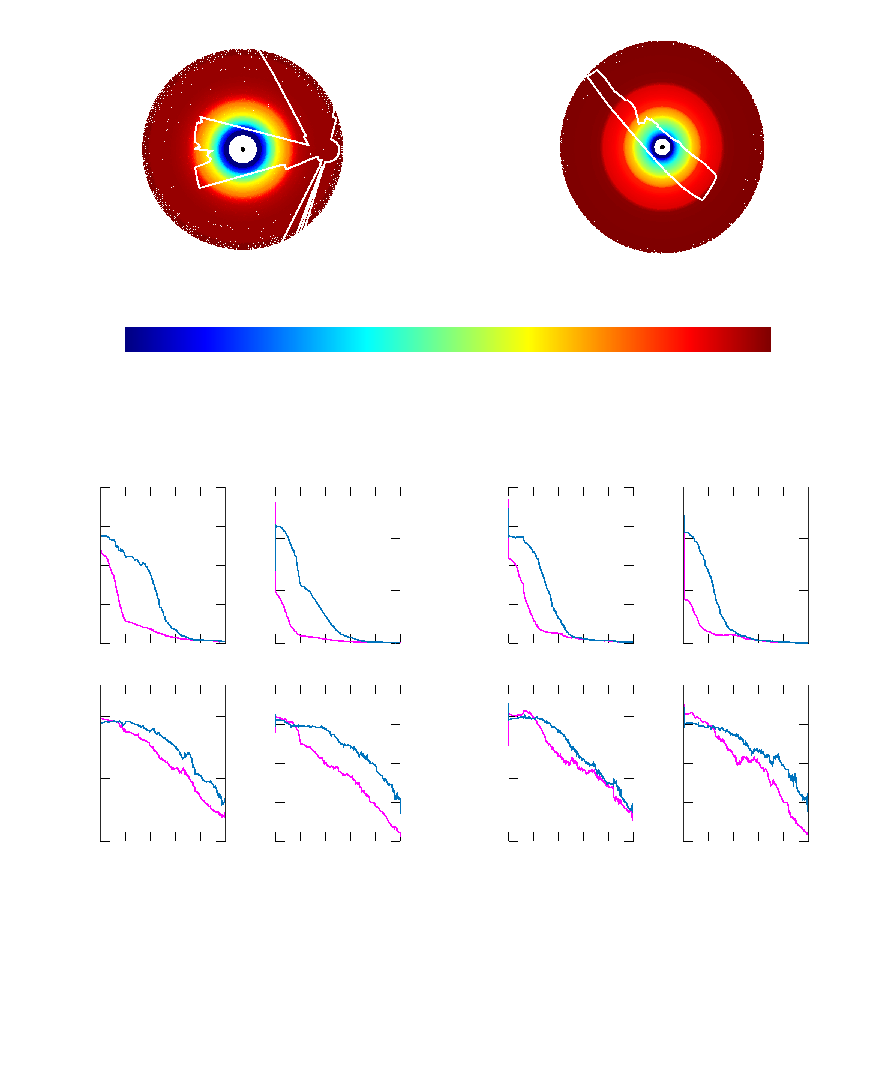
\includegraphics{./figures/parts/02/chapters/05/sections/04/max_range_test}}%
    \gplfronttext
  \end{picture}%
\endgroup

  \vspace{-2cm}
  \caption{\small Πειράματα απόκρισης του σφάλματος εκτίμησης των PLICP
           και FSM σε συνθήκες μειούμενου βεληνεκούς-μέγιστου εύρους
           για τυπική απόκλιση των διαταραχών που επιδρούν στις μετρήσεις του
           φυσικού αισθητήρα όταν $\sigma_R = 0.05$ m. Η διαμόρφωση
           $\Delta_\alpha: (\overline{\delta}_{xy}, \overline{\delta}_{\theta})
           = (0.05,0.174)$ [m,rad]. Η διαμόρφωση $\Delta_\beta:
           (\overline{\delta}_{xy},\overline{\delta}_{\theta}) = (0.20,\pi/4)$
           [m,rad]}
  \label{fig:02_05_04:04}
\end{figure}

Με βάση τα πειραματικά αποτελέσματα παρατηρούμε πως το σφάλμα εκτίμησης
προσανατολισμού του FSM είναι συγκρίσιμο με το ονομαστικό σε συνθήκες
όπου έως το $80\%$ των ακτίνων δεν φέρουν χωρική πληροφορία, σε αντίθεση με το
σφάλμα εκτίμησης θέσης, το οποίο είναι επί της αρχής αντιστρόφως ανάλογο του
ποσοστού των ακτίνων που φέρουν χωρική πληροφορία. Σε χαμηλότερα ποσοστά του
$80\%$ ο FSM επιδεικνύει χαμηλότερα σφάλματα εκτίμησης προσανατολισμού
από τον PLICP, ενώ τα σφάλματα εκτίμησης θέσης του γίνονται μεγαλύτερα από
εκείνα του PLICP όταν περίπου μόνο το $20\%$ των ακτίνων φέρουν ουσιαστική
πληροφορία, παρ' όλο που ο PLICP χρησιμοποιεί αντιστοιχίσεις (και συνεπώς θα
ήταν αναμενόμενο να είναι περισσότερο ικανός να αντιστοιχίσει μεμονωμένες
περιοχές των σαρώσεων μεταξύ τους).

Στο σχήμα \ref{fig:02_05_04:05} απεικονίζονται διαφορετικές όψεις της ευρωστίας
της μεθόδου FSM σε πραγματικές συνθήκες. Τα σχήματα της άνω σειράς
αναπαριστούν δύο αρχικές συνθήκες ευθυγράμμισης δισδιάστατων πανοραμικών
σαρώσεων, ενώ της μεσαίας τις τελικές ευθυγραμμίσεις που προέκυψαν μέσω της
εφαρμογής της FSM. Στην αριστερή συνθήκη η τυπική απόκλιση του θορύβου
μέτρησης είναι $\sigma_R = 0.05$ m, ενώ στη δεξιά $\sigma_R = 0.0$ m. Η
τελευταία σειρά εστιάζει σε σημεία ενδιαφέροντος, ήτοι σε περιοχές που εκθέτουν
την ευρωστία της μεθόδου ως προς το θόρυβο μέτρησης, αλλαγές περιβάλλοντος
απρόβλεπτου μέτρου, και ατελείς επικαλύψεις ανάμεσα στις εισόδους.

\begin{figure}[]\centering
  % GNUPLOT: LaTeX picture with Postscript
\begingroup
  \makeatletter
  \providecommand\color[2][]{%
    \GenericError{(gnuplot) \space\space\space\@spaces}{%
      Package color not loaded in conjunction with
      terminal option `colourtext'%
    }{See the gnuplot documentation for explanation.%
    }{Either use 'blacktext' in gnuplot or load the package
      color.sty in LaTeX.}%
    \renewcommand\color[2][]{}%
  }%
  \providecommand\includegraphics[2][]{%
    \GenericError{(gnuplot) \space\space\space\@spaces}{%
      Package graphicx or graphics not loaded%
    }{See the gnuplot documentation for explanation.%
    }{The gnuplot epslatex terminal needs graphicx.sty or graphics.sty.}%
    \renewcommand\includegraphics[2][]{}%
  }%
  \providecommand\rotatebox[2]{#2}%
  \@ifundefined{ifGPcolor}{%
    \newif\ifGPcolor
    \GPcolorfalse
  }{}%
  \@ifundefined{ifGPblacktext}{%
    \newif\ifGPblacktext
    \GPblacktexttrue
  }{}%
  % define a \g@addto@macro without @ in the name:
  \let\gplgaddtomacro\g@addto@macro
  % define empty templates for all commands taking text:
  \gdef\gplbacktext{}%
  \gdef\gplfronttext{}%
  \makeatother
  \ifGPblacktext
    % no textcolor at all
    \def\colorrgb#1{}%
    \def\colorgray#1{}%
  \else
    % gray or color?
    \ifGPcolor
      \def\colorrgb#1{\color[rgb]{#1}}%
      \def\colorgray#1{\color[gray]{#1}}%
      \expandafter\def\csname LTw\endcsname{\color{white}}%
      \expandafter\def\csname LTb\endcsname{\color{black}}%
      \expandafter\def\csname LTa\endcsname{\color{black}}%
      \expandafter\def\csname LT0\endcsname{\color[rgb]{1,0,0}}%
      \expandafter\def\csname LT1\endcsname{\color[rgb]{0,1,0}}%
      \expandafter\def\csname LT2\endcsname{\color[rgb]{0,0,1}}%
      \expandafter\def\csname LT3\endcsname{\color[rgb]{1,0,1}}%
      \expandafter\def\csname LT4\endcsname{\color[rgb]{0,1,1}}%
      \expandafter\def\csname LT5\endcsname{\color[rgb]{1,1,0}}%
      \expandafter\def\csname LT6\endcsname{\color[rgb]{0,0,0}}%
      \expandafter\def\csname LT7\endcsname{\color[rgb]{1,0.3,0}}%
      \expandafter\def\csname LT8\endcsname{\color[rgb]{0.5,0.5,0.5}}%
    \else
      % gray
      \def\colorrgb#1{\color{black}}%
      \def\colorgray#1{\color[gray]{#1}}%
      \expandafter\def\csname LTw\endcsname{\color{white}}%
      \expandafter\def\csname LTb\endcsname{\color{black}}%
      \expandafter\def\csname LTa\endcsname{\color{black}}%
      \expandafter\def\csname LT0\endcsname{\color{black}}%
      \expandafter\def\csname LT1\endcsname{\color{black}}%
      \expandafter\def\csname LT2\endcsname{\color{black}}%
      \expandafter\def\csname LT3\endcsname{\color{black}}%
      \expandafter\def\csname LT4\endcsname{\color{black}}%
      \expandafter\def\csname LT5\endcsname{\color{black}}%
      \expandafter\def\csname LT6\endcsname{\color{black}}%
      \expandafter\def\csname LT7\endcsname{\color{black}}%
      \expandafter\def\csname LT8\endcsname{\color{black}}%
    \fi
  \fi
    \setlength{\unitlength}{0.0500bp}%
    \ifx\gptboxheight\undefined%
      \newlength{\gptboxheight}%
      \newlength{\gptboxwidth}%
      \newsavebox{\gptboxtext}%
    \fi%
    \setlength{\fboxrule}{0.5pt}%
    \setlength{\fboxsep}{1pt}%
\begin{picture}(8000.00,12000.00)%
    \gplgaddtomacro\gplbacktext{%
      \colorrgb{0.15,0.15,0.15}%
      \put(-52,9611){\makebox(0,0)[r]{\strut{}$-32$}}%
      \colorrgb{0.15,0.15,0.15}%
      \put(-52,10173){\makebox(0,0)[r]{\strut{}$-24$}}%
      \colorrgb{0.15,0.15,0.15}%
      \put(-52,10734){\makebox(0,0)[r]{\strut{}$-16$}}%
      \colorrgb{0.15,0.15,0.15}%
      \put(-52,11296){\makebox(0,0)[r]{\strut{}$-8$}}%
      \colorrgb{0.15,0.15,0.15}%
      \put(-52,11857){\makebox(0,0)[r]{\strut{}$0$}}%
      \colorrgb{0.15,0.15,0.15}%
      \put(641,9321){\makebox(0,0){\strut{}$30$}}%
      \colorrgb{0.15,0.15,0.15}%
      \put(1343,9321){\makebox(0,0){\strut{}$50$}}%
      \colorrgb{0.15,0.15,0.15}%
      \put(2045,9321){\makebox(0,0){\strut{}$50$}}%
      \colorrgb{0.15,0.15,0.15}%
      \put(2746,9321){\makebox(0,0){\strut{}$60$}}%
      \colorrgb{0.15,0.15,0.15}%
      \put(3448,9321){\makebox(0,0){\strut{}$70$}}%
    }%
    \gplgaddtomacro\gplfronttext{%
      \colorrgb{0.00,0.00,0.00}%
      \put(1182,12050){\makebox(0,0)[l]{\strut{}Αρχική συνθήκη}}%
      \put(982,9000){\makebox(0,0)[l]{\strut{}$\Delta x = -0.03252$ m}}%
      \put(982,8750){\makebox(0,0)[l]{\strut{}$\Delta y = +0.03603$ m}}%
      \put(982,8500){\makebox(0,0)[l]{\strut{}$\Delta \theta = -0.35689$ rad}}%
    }%
    \gplgaddtomacro\gplbacktext{%
      \colorrgb{0.15,0.15,0.15}%
      \put(4748,9755){\makebox(0,0)[r]{\strut{}$-12$}}%
      \colorrgb{0.15,0.15,0.15}%
      \put(4748,10227){\makebox(0,0)[r]{\strut{}$-10$}}%
      \colorrgb{0.15,0.15,0.15}%
      \put(4748,10699){\makebox(0,0)[r]{\strut{}$-8$}}%
      \colorrgb{0.15,0.15,0.15}%
      \put(4748,11171){\makebox(0,0)[r]{\strut{}$-6$}}%
      \colorrgb{0.15,0.15,0.15}%
      \put(4748,11643){\makebox(0,0)[r]{\strut{}$-4$}}%
      \colorrgb{0.15,0.15,0.15}%
      \put(5116,9299){\makebox(0,0){\strut{}$28$}}%
      \colorrgb{0.15,0.15,0.15}%
      \put(5588,9299){\makebox(0,0){\strut{}$30$}}%
      \colorrgb{0.15,0.15,0.15}%
      \put(6060,9299){\makebox(0,0){\strut{}$32$}}%
      \colorrgb{0.15,0.15,0.15}%
      \put(6531,9299){\makebox(0,0){\strut{}$34$}}%
      \colorrgb{0.15,0.15,0.15}%
      \put(7003,9299){\makebox(0,0){\strut{}$36$}}%
    }%
    \gplgaddtomacro\gplfronttext{%
      \colorrgb{0.00,0.00,0.00}%
      \put(5300,12050){\makebox(0,0)[l]{\strut{}Αρχική συνθήκη}}%
      \put(5200,9000){\makebox(0,0)[l]{\strut{}$\Delta x = -0.02856$ m}}%
      \put(5200,8750){\makebox(0,0)[l]{\strut{}$\Delta y = -0.19805$ m}}%
      \put(5200,8500){\makebox(0,0)[l]{\strut{}$\Delta \theta = -1.31500$ rad}}%
    }%
    \gplgaddtomacro\gplbacktext{%
      \colorrgb{0.15,0.15,0.15}%
      \put(-52,6118){\makebox(0,0)[r]{\strut{}$-32$}}%
      \colorrgb{0.15,0.15,0.15}%
      \put(-52,6399){\makebox(0,0)[r]{\strut{}$-28$}}%
      \colorrgb{0.15,0.15,0.15}%
      \put(-52,6679){\makebox(0,0)[r]{\strut{}$-24$}}%
      \colorrgb{0.15,0.15,0.15}%
      \put(-52,6960){\makebox(0,0)[r]{\strut{}$-20$}}%
      \colorrgb{0.15,0.15,0.15}%
      \put(641,5828){\makebox(0,0){\strut{}$30$}}%
      \colorrgb{0.15,0.15,0.15}%
      \put(1343,5828){\makebox(0,0){\strut{}$50$}}%
      \colorrgb{0.15,0.15,0.15}%
      \put(2045,5828){\makebox(0,0){\strut{}$50$}}%
      \colorrgb{0.15,0.15,0.15}%
      \put(2746,5828){\makebox(0,0){\strut{}$60$}}%
      \colorrgb{0.15,0.15,0.15}%
      \put(3448,5828){\makebox(0,0){\strut{}$70$}}%
    }%
    \gplgaddtomacro\gplfronttext{%
      \colorrgb{0.00,0.00,0.00}%
      \put(982,7200){\makebox(0,0)[l]{\strut{}Τελική ευθυγράμμιση}}%
      \put(982,5500){\makebox(0,0)[l]{\strut{}$\Delta x = -0.00085$ m}}%
      \put(982,5250){\makebox(0,0)[l]{\strut{}$\Delta y = +0.00337$ m}}%
      \put(982,5000){\makebox(0,0)[l]{\strut{}$\Delta \theta = -0.00346$ rad}}%
    }%
    \gplgaddtomacro\gplbacktext{%
      \colorrgb{0.15,0.15,0.15}%
      \put(4748,5596){\makebox(0,0)[r]{\strut{}$-12$}}%
      \colorrgb{0.15,0.15,0.15}%
      \put(4748,6068){\makebox(0,0)[r]{\strut{}$-10$}}%
      \colorrgb{0.15,0.15,0.15}%
      \put(4748,6540){\makebox(0,0)[r]{\strut{}$-8$}}%
      \colorrgb{0.15,0.15,0.15}%
      \put(4748,7011){\makebox(0,0)[r]{\strut{}$-6$}}%
      \colorrgb{0.15,0.15,0.15}%
      \put(4748,7483){\makebox(0,0)[r]{\strut{}$-4$}}%
      \colorrgb{0.15,0.15,0.15}%
      \put(5116,5140){\makebox(0,0){\strut{}$28$}}%
      \colorrgb{0.15,0.15,0.15}%
      \put(5588,5140){\makebox(0,0){\strut{}$30$}}%
      \colorrgb{0.15,0.15,0.15}%
      \put(6060,5140){\makebox(0,0){\strut{}$32$}}%
      \colorrgb{0.15,0.15,0.15}%
      \put(6531,5140){\makebox(0,0){\strut{}$34$}}%
      \colorrgb{0.15,0.15,0.15}%
      \put(7003,5140){\makebox(0,0){\strut{}$36$}}%
    }%
    \gplgaddtomacro\gplfronttext{%
      \colorrgb{0.00,0.00,0.00}%
      \put(5100,7900){\makebox(0,0)[l]{\strut{}Τελική ευθυγράμμιση}}%
      \put(5200,4800){\makebox(0,0)[l]{\strut{}$\Delta x = +0.00643$ m}}%
      \put(5200,4550){\makebox(0,0)[l]{\strut{}$\Delta y = +0.00371$ m}}%
      \put(5200,4300){\makebox(0,0)[l]{\strut{}$\Delta \theta = +0.00194$ rad}}%
    }%
    \gplgaddtomacro\gplbacktext{%
      \colorrgb{0.15,0.15,0.15}%
      \put(42,1815){\makebox(0,0)[r]{\strut{}\scriptsize $-26$}}%
      \colorrgb{0.15,0.15,0.15}%
      \put(42,2479){\makebox(0,0)[r]{\strut{}\scriptsize $-25$}}%
      \colorrgb{0.15,0.15,0.15}%
      \put(42,3143){\makebox(0,0)[r]{\strut{}\scriptsize $-24$}}%
      \colorrgb{0.15,0.15,0.15}%
      \put(412,1263){\makebox(0,0){\strut{}\scriptsize $26$}}%
      \colorrgb{0.15,0.15,0.15}%
      \put(1075,1263){\makebox(0,0){\strut{}\scriptsize $27$}}%
      \colorrgb{0.15,0.15,0.15}%
      \put(1739,1263){\makebox(0,0){\strut{}\scriptsize $28$}}%
    }%
    \gplgaddtomacro\gplfronttext{%
      \colorrgb{0.00,0.00,0.00}%
      \put(909,3496){\makebox(0,0){\strut{}Θόρυβος μέτρησης}}%
    }%
    \gplgaddtomacro\gplbacktext{%
      \colorrgb{0.15,0.15,0.15}%
      \put(2108,2073){\makebox(0,0)[r]{\strut{}\scriptsize $-25$}}%
      \colorrgb{0.15,0.15,0.15}%
      \put(2108,2364){\makebox(0,0)[r]{\strut{}\scriptsize $-24$}}%
      \colorrgb{0.15,0.15,0.15}%
      \put(2108,2656){\makebox(0,0)[r]{\strut{}\scriptsize $-23$}}%
      \colorrgb{0.15,0.15,0.15}%
      \put(2518,1635){\makebox(0,0){\strut{}\scriptsize $31$}}%
      \colorrgb{0.15,0.15,0.15}%
      \put(3100,1635){\makebox(0,0){\strut{}\scriptsize $33$}}%
      \colorrgb{0.15,0.15,0.15}%
      \put(3683,1635){\makebox(0,0){\strut{}\scriptsize $35$}}%
    }%
    \gplgaddtomacro\gplfronttext{%
    }%
    \gplgaddtomacro\gplbacktext{%
      \colorrgb{0.15,0.15,0.15}%
      \put(4168,1901){\makebox(0,0)[r]{\strut{}\scriptsize $-6$}}%
      \colorrgb{0.15,0.15,0.15}%
      \put(4168,2464){\makebox(0,0)[r]{\strut{}\scriptsize $-5$}}%
      \colorrgb{0.15,0.15,0.15}%
      \put(4168,3027){\makebox(0,0)[r]{\strut{}\scriptsize $-4$}}%
      \colorrgb{0.15,0.15,0.15}%
      \put(4706,1231){\makebox(0,0){\strut{}\scriptsize $32$}}%
      \colorrgb{0.15,0.15,0.15}%
      \put(5269,1231){\makebox(0,0){\strut{}\scriptsize $33$}}%
      \colorrgb{0.15,0.15,0.15}%
      \put(5831,1231){\makebox(0,0){\strut{}\scriptsize $34$}}%
    }%
    \gplgaddtomacro\gplfronttext{%
      \colorrgb{0.00,0.00,0.00}%
      \put(2457,3589){\makebox(0,0)[l]{\strut{}Στοιχεία υψηλής συχνότητος}}%
    }%
    \gplgaddtomacro\gplbacktext{%
      \colorrgb{0.15,0.15,0.15}%
      \put(6228,1704){\makebox(0,0)[r]{\strut{}\scriptsize $-8$}}%
      \colorrgb{0.15,0.15,0.15}%
      \put(6228,2165){\makebox(0,0)[r]{\strut{}\scriptsize $-7$}}%
      \colorrgb{0.15,0.15,0.15}%
      \put(6228,2626){\makebox(0,0)[r]{\strut{}\scriptsize $-6$}}%
      \colorrgb{0.15,0.15,0.15}%
      \put(6228,3087){\makebox(0,0)[r]{\strut{}\scriptsize $-5$}}%
      \colorrgb{0.15,0.15,0.15}%
      \put(6260,1406){\makebox(0,0){\strut{}\scriptsize $30$}}%
      \colorrgb{0.15,0.15,0.15}%
      \put(6721,1406){\makebox(0,0){\strut{}\scriptsize $31$}}%
      \colorrgb{0.15,0.15,0.15}%
      \put(7182,1406){\makebox(0,0){\strut{}\scriptsize $32$}}%
      \colorrgb{0.15,0.15,0.15}%
      \put(7643,1406){\makebox(0,0){\strut{}\scriptsize $33$}}%
    }%
    \gplgaddtomacro\gplfronttext{%
      \colorrgb{0.00,0.00,0.00}%
      \put(7089,3353){\makebox(0,0){\strut{}Απούσες αντιστοιχίες}}%
    }%
    \gplbacktext
    \put(0,0){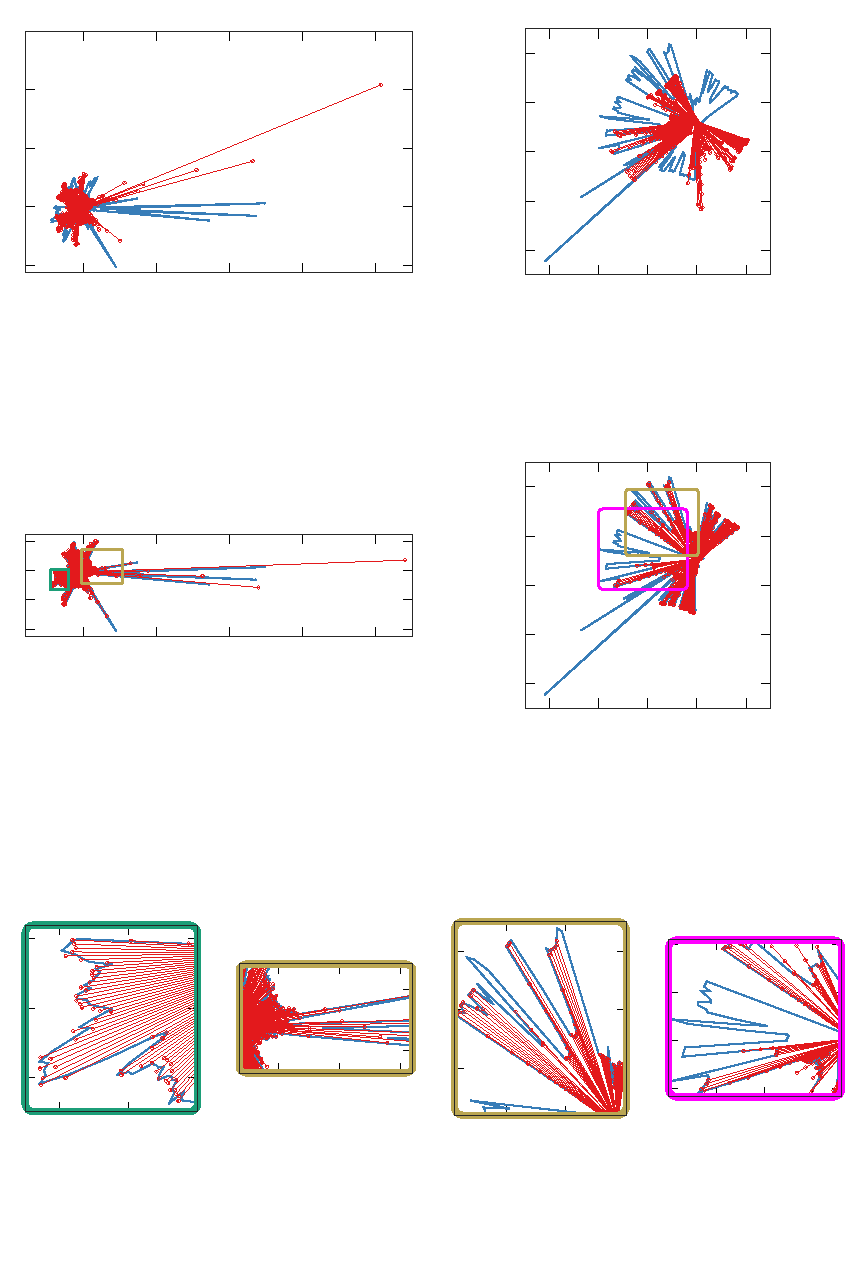
\includegraphics{./figures/parts/02/chapters/05/sections/04/from_video}}%
    \gplfronttext
  \end{picture}%
\endgroup

  \vspace{-1cm}
  \caption{\small Παραδείγματα ευθυγράμμισης σαρώσεων που εκθέτουν τις αρετές
           του FSM σε καταστάσεις πραγματικών συνθηκών: ο FSM
           είναι ταυτόχρονα εύρωστος σε θόρυβο μέτρησης, απρόβλεπτα μεγάλες
           αλλαγές στο περιβάλλον από το οποίο συλλαμβάνονται οι σαρώσεις
           εισόδου του, και σε συνθήκες μερικής επικάλυψης}
  \label{fig:02_05_04:05}
\end{figure}
